\section{Dự đoán tỷ lệ tội phạm bạo lực trong các cộng đồng ở Hoa Kỳ dựa trên các đặc điểm nhân khẩu học, kinh tế và xã hội.}

% Thành viên Nguyễn Nhật Quang điền nội dung tại đây.
\subsection{Giới thiệu và đề
bài}\label{giux1edbi-thiux1ec7u-vuxe0-ux111ux1ec1-buxe0i}

\subsubsection{Bối cảnh và mục
tiêu}\label{bux1ed1i-cux1ea3nh-vuxe0-mux1ee5c-tiuxeau}

Bài toán là \textbf{dự đoán tỷ lệ tội phạm bạo lực trên đầu người}
(\texttt{ViolentCrimesPerPop}) của các cộng đồng Hoa Kỳ từ hơn 100 biến
kinh tế, xã hội, nhà ở và cảnh sát. Dựa trên mô tả của bộ dữ liệu, nhiều
biến đo gần cùng một hiện tượng, nên đa cộng tuyến là vấn đề trung tâm
cần xử lý.

Báo cáo tập trung vào \textbf{hồi quy trên thành phần chính} và so sánh
công bằng với các mô hình hồi quy khác: \textbf{OLS}, \textbf{Ridge} và
\textbf{LASSO}.

\subsubsection{Quy trình phân tích}\label{quy-truxecnh-phuxe2n-tuxedch}

Báo cáo được tổ chức theo đúng trình tự yêu cầu của đề bài:

\begin{enumerate}
\def\labelenumi{\arabic{enumi}.}
\tightlist
\item
  \textbf{Khám phá dữ liệu (EDA)}: Tìm hiểu phân phối biến phản hồi, cấu
  trúc dữ liệu khuyết, chẩn đoán hiện tượng đa cộng tuyến và đưa ra các
  giả thuyết về quá trình sinh dữ liệu cũng như insight
\item
  \textbf{Tiền xử lý}: đưa ra các quyết định xử lý dữ liệu dựa trên kết
  quả EDA, mỗi quyết định đi kèm lý do thống kê cụ thể;
\item
  \textbf{Chia dữ liệu}: Chia dữ liệu thành tập huấn luyện và tập kiểm
  định để đo lường tính hiệu quả của mô hình
\item
  \textbf{Xây dựng mô hình PCR}: Kiểm tra mức độ phù hợp của dữ liệu với
  PCR, lựa chọn số thành phần chính, xây dựng mô hình hồi quy trên thành
  phần chính;
\item
  \textbf{Các mô hình đối chứng}: Kiểm tra mức độ phù hợp của các mô
  hình OLS, Ridge, LASSO. Xây dựng mô hình hồi quy và đánh giá kết quả
  của các mô hình hồi quy này.
\item
  \textbf{Đánh giá và so sánh}: Đánh giá và so sánh kết quả của các mô
  hình hồi quy trên tập kiểm định bằng RMSE, MAE, \(R^2\);
\item
  \textbf{Phân tích ma trận tải (loadings)} và \textbf{chuyển hệ số PCR
  về không gian biến gốc};
\item
  \textbf{Thảo luận, lựa chọn mô hình và kết luận}.
\end{enumerate}

\subsection{Bộ dữ liệu}\label{bux1ed9-dux1eef-liux1ec7u}

\subsubsection{Nguồn gốc}\label{nguux1ed3n-gux1ed1c}

Bộ dữ liệu sử dụng trong báo cáo là tập tin \texttt{communities.data} do
giảng viên cung cấp. Theo nội dung đề bài và tài liệu mô tả
\texttt{communities.names} đi kèm, đây là bộ dữ liệu \textbf{Communities
and Crime} được công bố trên UCI Machine Learning Repository. Bộ dữ liệu
được tổng hợp từ ba nguồn:

\begin{itemize}
\tightlist
\item
  \textbf{Điều tra dân số Hoa Kỳ năm 1990} (\emph{1990 U.S. Census}):
  Bao gồm các biến kinh tế xã hội và nhân khẩu học;
\item
  \textbf{Khảo sát LEMAS 1990} (\emph{Law Enforcement Management and
  Administrative Statistics}): Bao gồm các biến về tổ chức và nguồn lực
  cảnh sát;
\item
  \textbf{Báo cáo tội phạm FBI UCR 1995} (\emph{Uniform Crime Reports}):
  Bao gồm biến phản hồi về tội phạm bạo lực.
\end{itemize}

Mỗi quan sát tương ứng với một cộng đồng ở Mỹ. Theo tài liệu mô tả
\texttt{communities.names}, bộ dữ liệu gồm \textbf{1994 quan sát và 128
biến}. Trong đó, \texttt{state}, \texttt{county}, \texttt{community} và
\texttt{communityname} là \textbf{4 biến định danh}; \texttt{fold} là
biến chỉ định phân hoạch kiểm chứng chéo do tác giả bộ dữ liệu tạo sẵn,
không được sử dụng làm biến dự báo. Sau khi loại 4 biến định danh và
biến \texttt{fold}, dữ liệu còn \textbf{122 biến dự báo} và \textbf{1
biến mục tiêu} \texttt{ViolentCrimesPerPop}.

Một đặc điểm rất quan trọng của bộ dữ liệu, được ghi rõ trong tài liệu:
\textbf{tất cả các biến dự báo dạng số và biến phản hồi đã được tác giả
đưa về thang \([0, 1]\) bằng phương pháp chia khoảng đều} với giá trị
ngoài khoảng \(\pm 3\) độ lệch chuẩn bị cắt về 0 hoặc 1.

\subsubsection{Các nhóm biến}\label{cuxe1c-nhuxf3m-biux1ebfn}

122 biến dự báo có thể chia thành các nhóm nội dung sau (bảng này sẽ
được dùng lại khi diễn giải các thành phần chính ở phần phân tích ma
trận tải):

\begin{landscape}
\small
\begin{longtable}[t]{
  >{\raggedright\arraybackslash}p{0.20\linewidth}
  >{\centering\arraybackslash}p{0.06\linewidth}
  >{\raggedright\arraybackslash}p{0.34\linewidth}
  >{\raggedright\arraybackslash}p{0.32\linewidth}}
\caption{\label{tab:bang-nhom-bien}Các nhóm nội dung của 122 biến dự báo.}\\
\toprule
Nhóm biến & Số biến & Ví dụ tiêu biểu & Nội dung\\
\midrule
Nhân khẩu học \& đô thị hóa & 12 & population, racePctWhite, agePct12t21, pctUrban & Quy mô dân số, cơ cấu chủng tộc, cơ cấu tuổi, mức độ đô thị hóa\\
Thu nhập \& nghèo đói & 17 & medIncome, perCapInc, pctWPubAsst, PctPopUnderPov & Thu nhập hộ/đầu người, nguồn thu nhập, trợ cấp xã hội, tỷ lệ nghèo\\
Giáo dục \& việc làm & 9 & PctNotHSGrad, PctBSorMore, PctUnemployed, PctOccupMgmtProf & Trình độ học vấn, thất nghiệp, cơ cấu nghề nghiệp\\
Cấu trúc gia đình & 13 & TotalPctDiv, PctFam2Par, PctKids2Par, PctIlleg & Ly hôn, gia đình đủ hai bố mẹ, con ngoài giá thú\\
Nhập cư \& ngôn ngữ & 11 & NumImmig, PctRecentImmig, PctNotSpeakEnglWell & Quy mô và mật độ nhập cư, khả năng tiếng Anh\\
\addlinespace
Nhà ở & 27 & PctPersDenseHous, HousVacant, OwnOccMedVal, MedRent & Mật độ ở, nhà trống, giá trị nhà, tiền thuê, chất lượng nhà ở\\
Vô gia cư \& ổn định cư trú & 7 & NumInShelters, NumStreet, PctSameHouse85, PctForeignBorn & Người vô gia cư, mức độ ổn định chỗ ở qua các năm\\
Cảnh sát (LEMAS) & 23 & LemasSwFTPerPop, PolicPerPop, PolicBudgPerPop & Quân số, ngân sách, tổ chức lực lượng cảnh sát\\
Địa lý khác & 3 & LandArea, PopDens, PctUsePubTrans & Diện tích, mật độ dân số, giao thông công cộng\\
\bottomrule
\end{longtable}
\end{landscape}

\subsection{Thực hiện phân tích dữ
liệu}\label{thux1ef1c-hiux1ec7n-phuxe2n-tuxedch-dux1eef-liux1ec7u}

\subsubsection{Phân phối của biến mục
tiêu}\label{phuxe2n-phux1ed1i-cux1ee7a-biux1ebfn-mux1ee5c-tiuxeau}

Trước hết ta khảo sát phân phối của biến mục tiêu \texttt{ViolentCrimesPerPop}.

\begin{longtable}[t]{rrrrrr}
\caption{\label{tab:phan-phoi-y}Thống kê mô tả của ViolentCrimesPerPop.}\\
\toprule
Trung bình & Trung vị & Độ lệch chuẩn & Skewness & Số quan sát y = 0 & Số quan sát y = 1\\
\midrule
0.238 & 0.15 & 0.233 & 1.52 & 10 & 44\\
\bottomrule
\end{longtable}

\begin{center}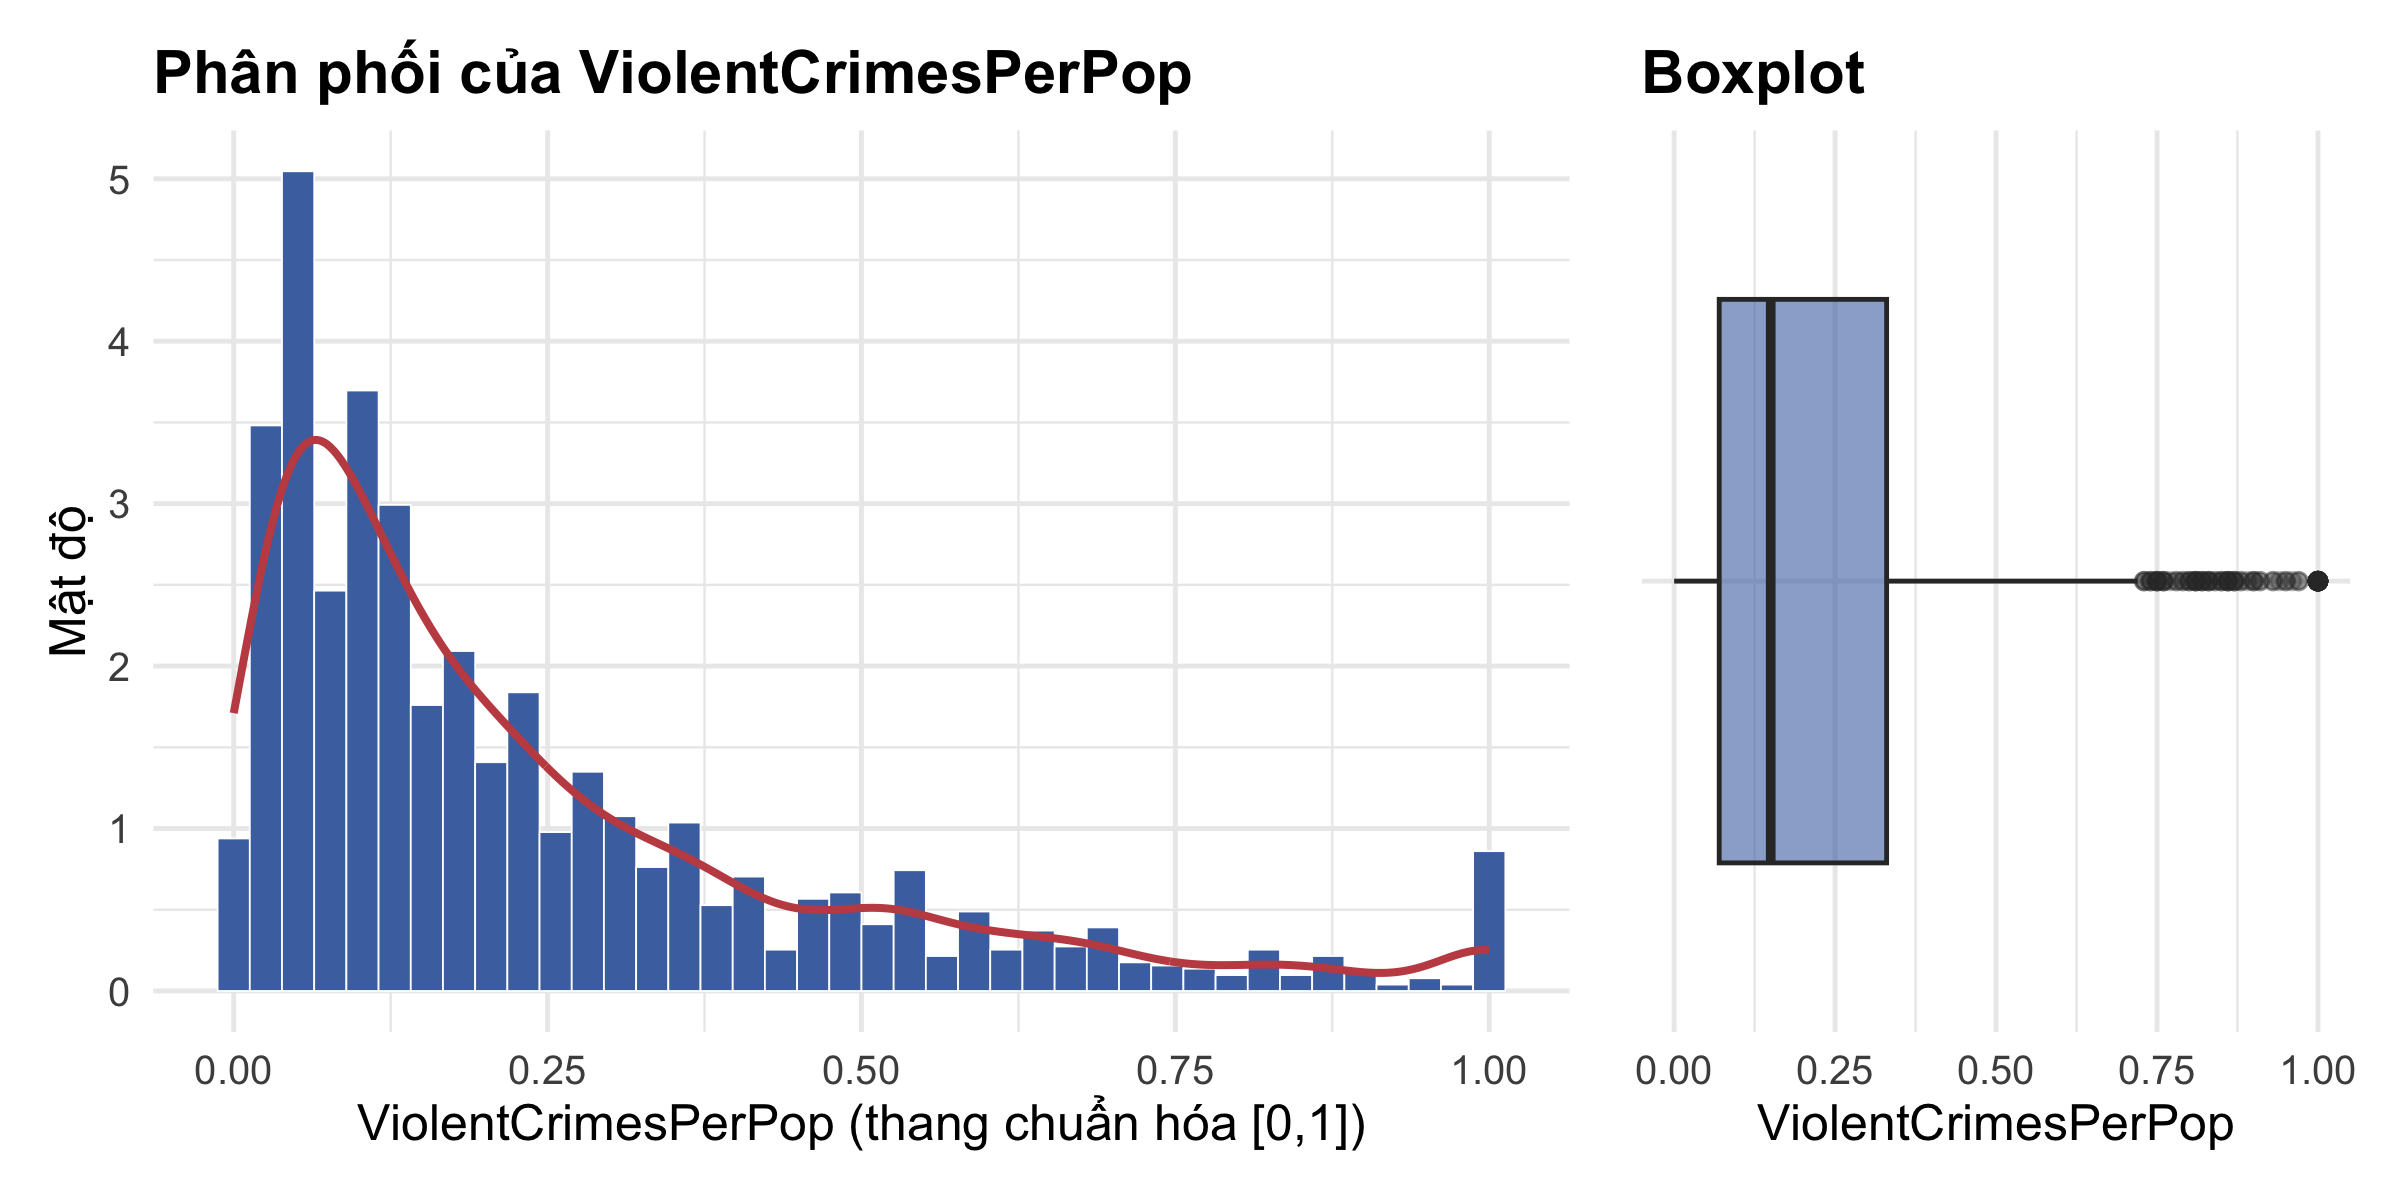
\includegraphics[width=\linewidth,keepaspectratio]{img/crime-phan-phoi-y-1.png} \end{center}

\textbf{Nhận xét.} Phân phối của biến phản hồi lệch phải: \(g_1=1.52\),
trung bình lớn hơn trung vị. Có 44 quan sát (2.2\%) tại trần 1 do quy
trình chuẩn hóa trước khi đưa vào mô hình hồi quy như những gì tác giả
mô tả trong tài liệu về việc thực hiện cap ở 2 đầu 0 và 1. Điều này làm
mất thứ tự giữa các giá trị gốc vượt ngưỡng và góp phần khiến mô hình
khó khớp vùng biên do đó không thể từ đó suy ra một trần \(R^2\) cụ thể.

\subsubsection{Phân tích về dữ liệu
khuyết}\label{phuxe2n-tuxedch-vux1ec1-dux1eef-liux1ec7u-khuyux1ebft}

Ta thống kê số giá trị khuyết theo từng biến và khảo sát xem chúng có
cấu trúc gì đặc biệt hay không vì để hiểu được \textbf{cơ chế sinh dữ
liệu khuyết}. Từ đó giúp chúng ta đưa ra được chiến lược phù hợp hơn để
giải quyết các biến này

\begin{longtable}[t]{lrr}
\caption{\label{tab:missing-tab}Top 10 biến có tỷ lệ khuyết cao nhất.}\\
\toprule
Biến & Số NA & Tỷ lệ (\%)\\
\midrule
LemasSwornFT & 1675 & 84\\
LemasSwFTPerPop & 1675 & 84\\
LemasSwFTFieldOps & 1675 & 84\\
LemasSwFTFieldPerPop & 1675 & 84\\
LemasTotalReq & 1675 & 84\\
\addlinespace
LemasTotReqPerPop & 1675 & 84\\
PolicReqPerOffic & 1675 & 84\\
PolicPerPop & 1675 & 84\\
RacialMatchCommPol & 1675 & 84\\
PctPolicWhite & 1675 & 84\\
\bottomrule
\end{longtable}

\begin{center}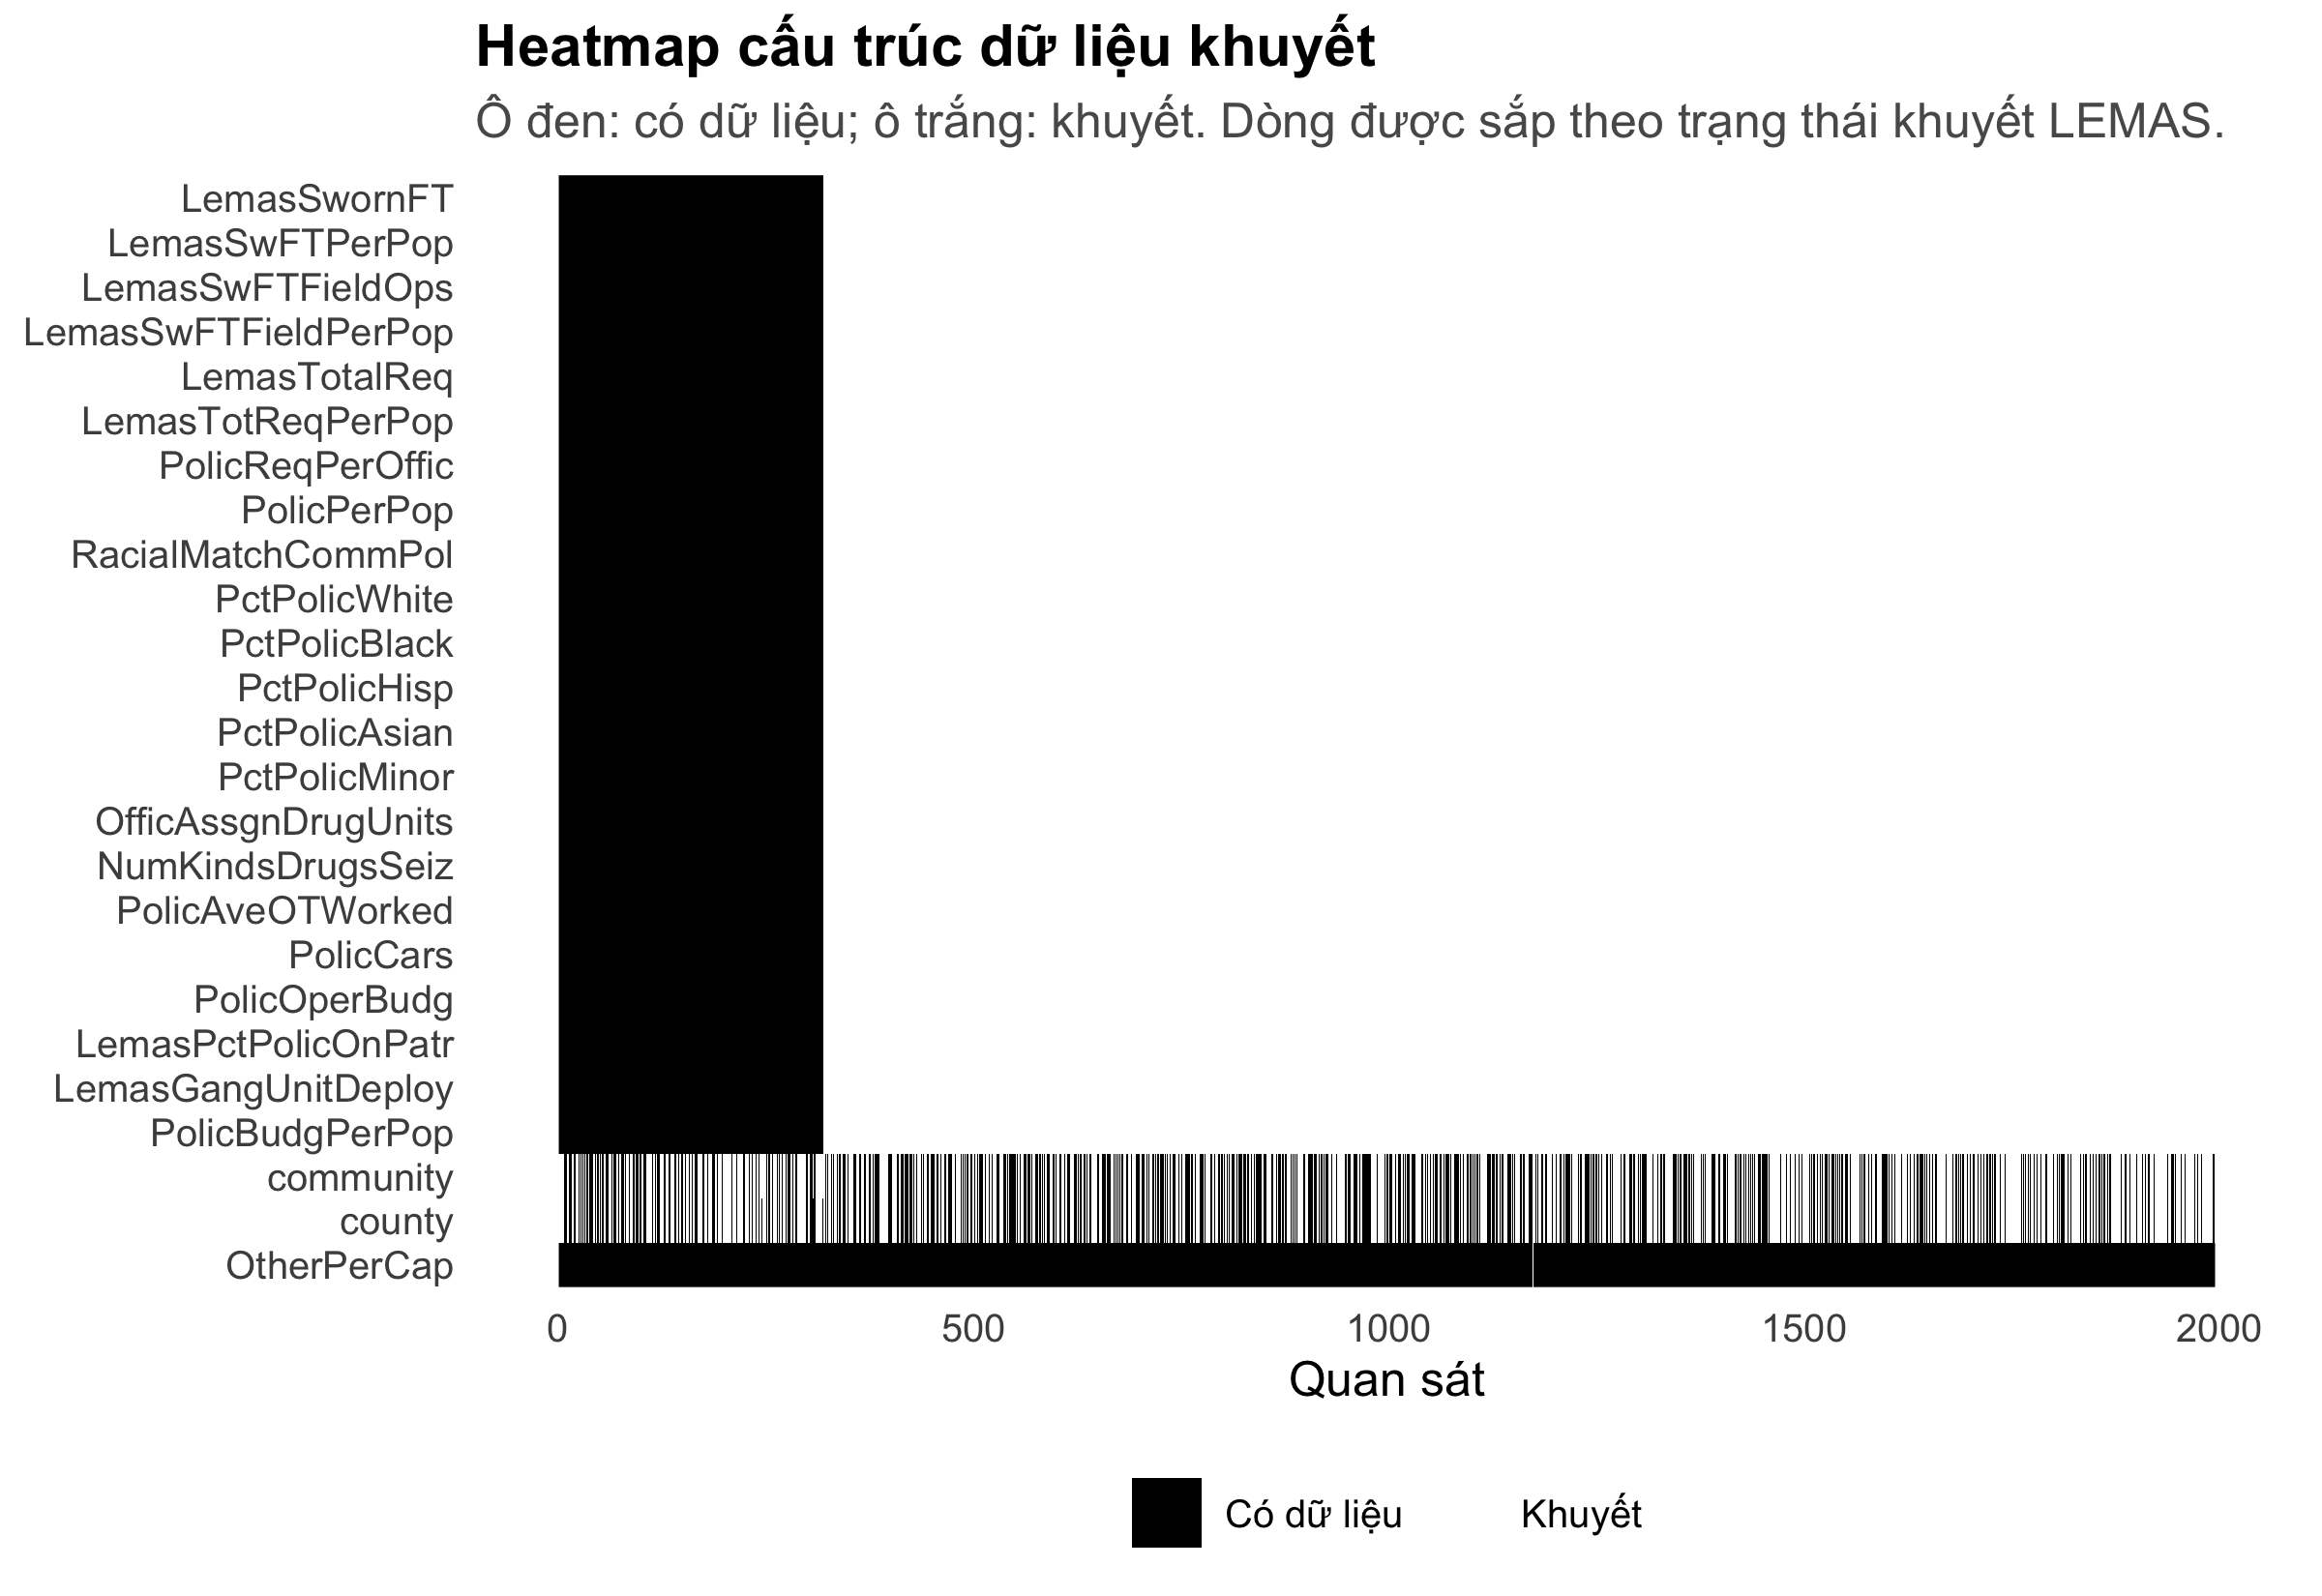
\includegraphics[width=\linewidth,keepaspectratio]{img/crime-missing-plot-1.png} \end{center}

Toàn bộ 22 biến khuyết nặng đều thuộc nhóm \textbf{cảnh sát (LEMAS)} và
cùng khuyết \textbf{đúng 1675 dòng như nhau}, điều này gợi ý rằng
missing data của ta có thể tuân theo một quy luật nhất định chứ không
rải rác ngẫu nhiên, lấy ví dụ như một cộng đồng hoặc có đầy đủ cả khối
biến LEMAS, hoặc không có biến nào. Để tìm nguyên nhân, ta so sánh quy
mô dân số giữa hai nhóm:

\begin{longtable}[t]{lrrr}
\caption{\label{tab:missing-pattern}So sánh quy mô dân số (thang chuẩn hóa) giữa nhóm có / khuyết dữ liệu LEMAS.}\\
\toprule
Nhóm & Số cộng đồng & Trung vị population & Trung bình population\\
\midrule
Có dữ liệu LEMAS & 319 & 0.14 & 0.229\\
Khuyết khối LEMAS & 1675 & 0.02 & 0.025\\
\bottomrule
\end{longtable}

\textbf{Nhận xét.} Xác suất khuyết LEMAS thay đổi rõ theo
\texttt{population}, nên dữ liệu cung cấp bằng chứng chống lại giả định
\textbf{MCAR} (khuyết hoàn toàn ngẫu nhiên). Mẫu hình này phù hợp với cơ
chế \textbf{MAR} có điều kiện theo quy mô cộng đồng.

Do 22 biến LEMAS cùng khuyết theo khối ở 84\% quan sát, do đó mà việc
xóa bỏ các dòng có giá trị khuyết sẽ làm mất phần lớn mẫu, còn
imputation sẽ phải ngoại suy từ 16\% cộng đồng có dữ liệu, chủ yếu là
cộng đồng lớn. Vì vậy, trong phạm vi báo cáo này, ta loại cả khối LEMAS
là lựa chọn đơn giản và thận trọng. Ngoài khối này, chỉ
\texttt{OtherPerCap} khuyết một giá trị; \texttt{county} và
\texttt{community} là biến định danh nên không được đưa trực tiếp vào mô
hình hồi quy.

\subsubsection{Tương quan giữa các biến và với biến phản
hồi}\label{tux1b0ux1a1ng-quan-giux1eefa-cuxe1c-biux1ebfn-vuxe0-vux1edbi-biux1ebfn-phux1ea3n-hux1ed3i}

Từ đây, để khảo sát cấu trúc tương quan, ta làm việc trên tập biến dự
báo sẽ được chốt chính thức ở phần tiền xử lý (bỏ 5 biến non-predictive
và khối LEMAS khuyết 84\%; giá trị khuyết duy nhất của
\texttt{OtherPerCap} được thay tạm bằng trung vị): ma trận
\(\mathbf{X}\) gồm \(100\) biến, \(n = 1994\) quan sát.

\begin{verbatim}
## [1] 1994  100
\end{verbatim}

\begin{longtable}[t]{lr}
\caption{\label{tab:cor-voi-y}15 biến tương quan mạnh nhất với ViolentCrimesPerPop.}\\
\toprule
Biến & Tương quan với y\\
\midrule
PctKids2Par & -0.738\\
PctIlleg & 0.738\\
PctFam2Par & -0.707\\
racePctWhite & -0.685\\
PctYoungKids2Par & -0.666\\
\addlinespace
PctTeen2Par & -0.662\\
racepctblack & 0.631\\
pctWInvInc & -0.576\\
pctWPubAsst & 0.575\\
FemalePctDiv & 0.556\\
\addlinespace
TotalPctDiv & 0.553\\
PctPersOwnOccup & -0.525\\
MalePctDivorce & 0.525\\
PctPopUnderPov & 0.522\\
PctUnemployed & 0.504\\
\bottomrule
\end{longtable}

\begin{center}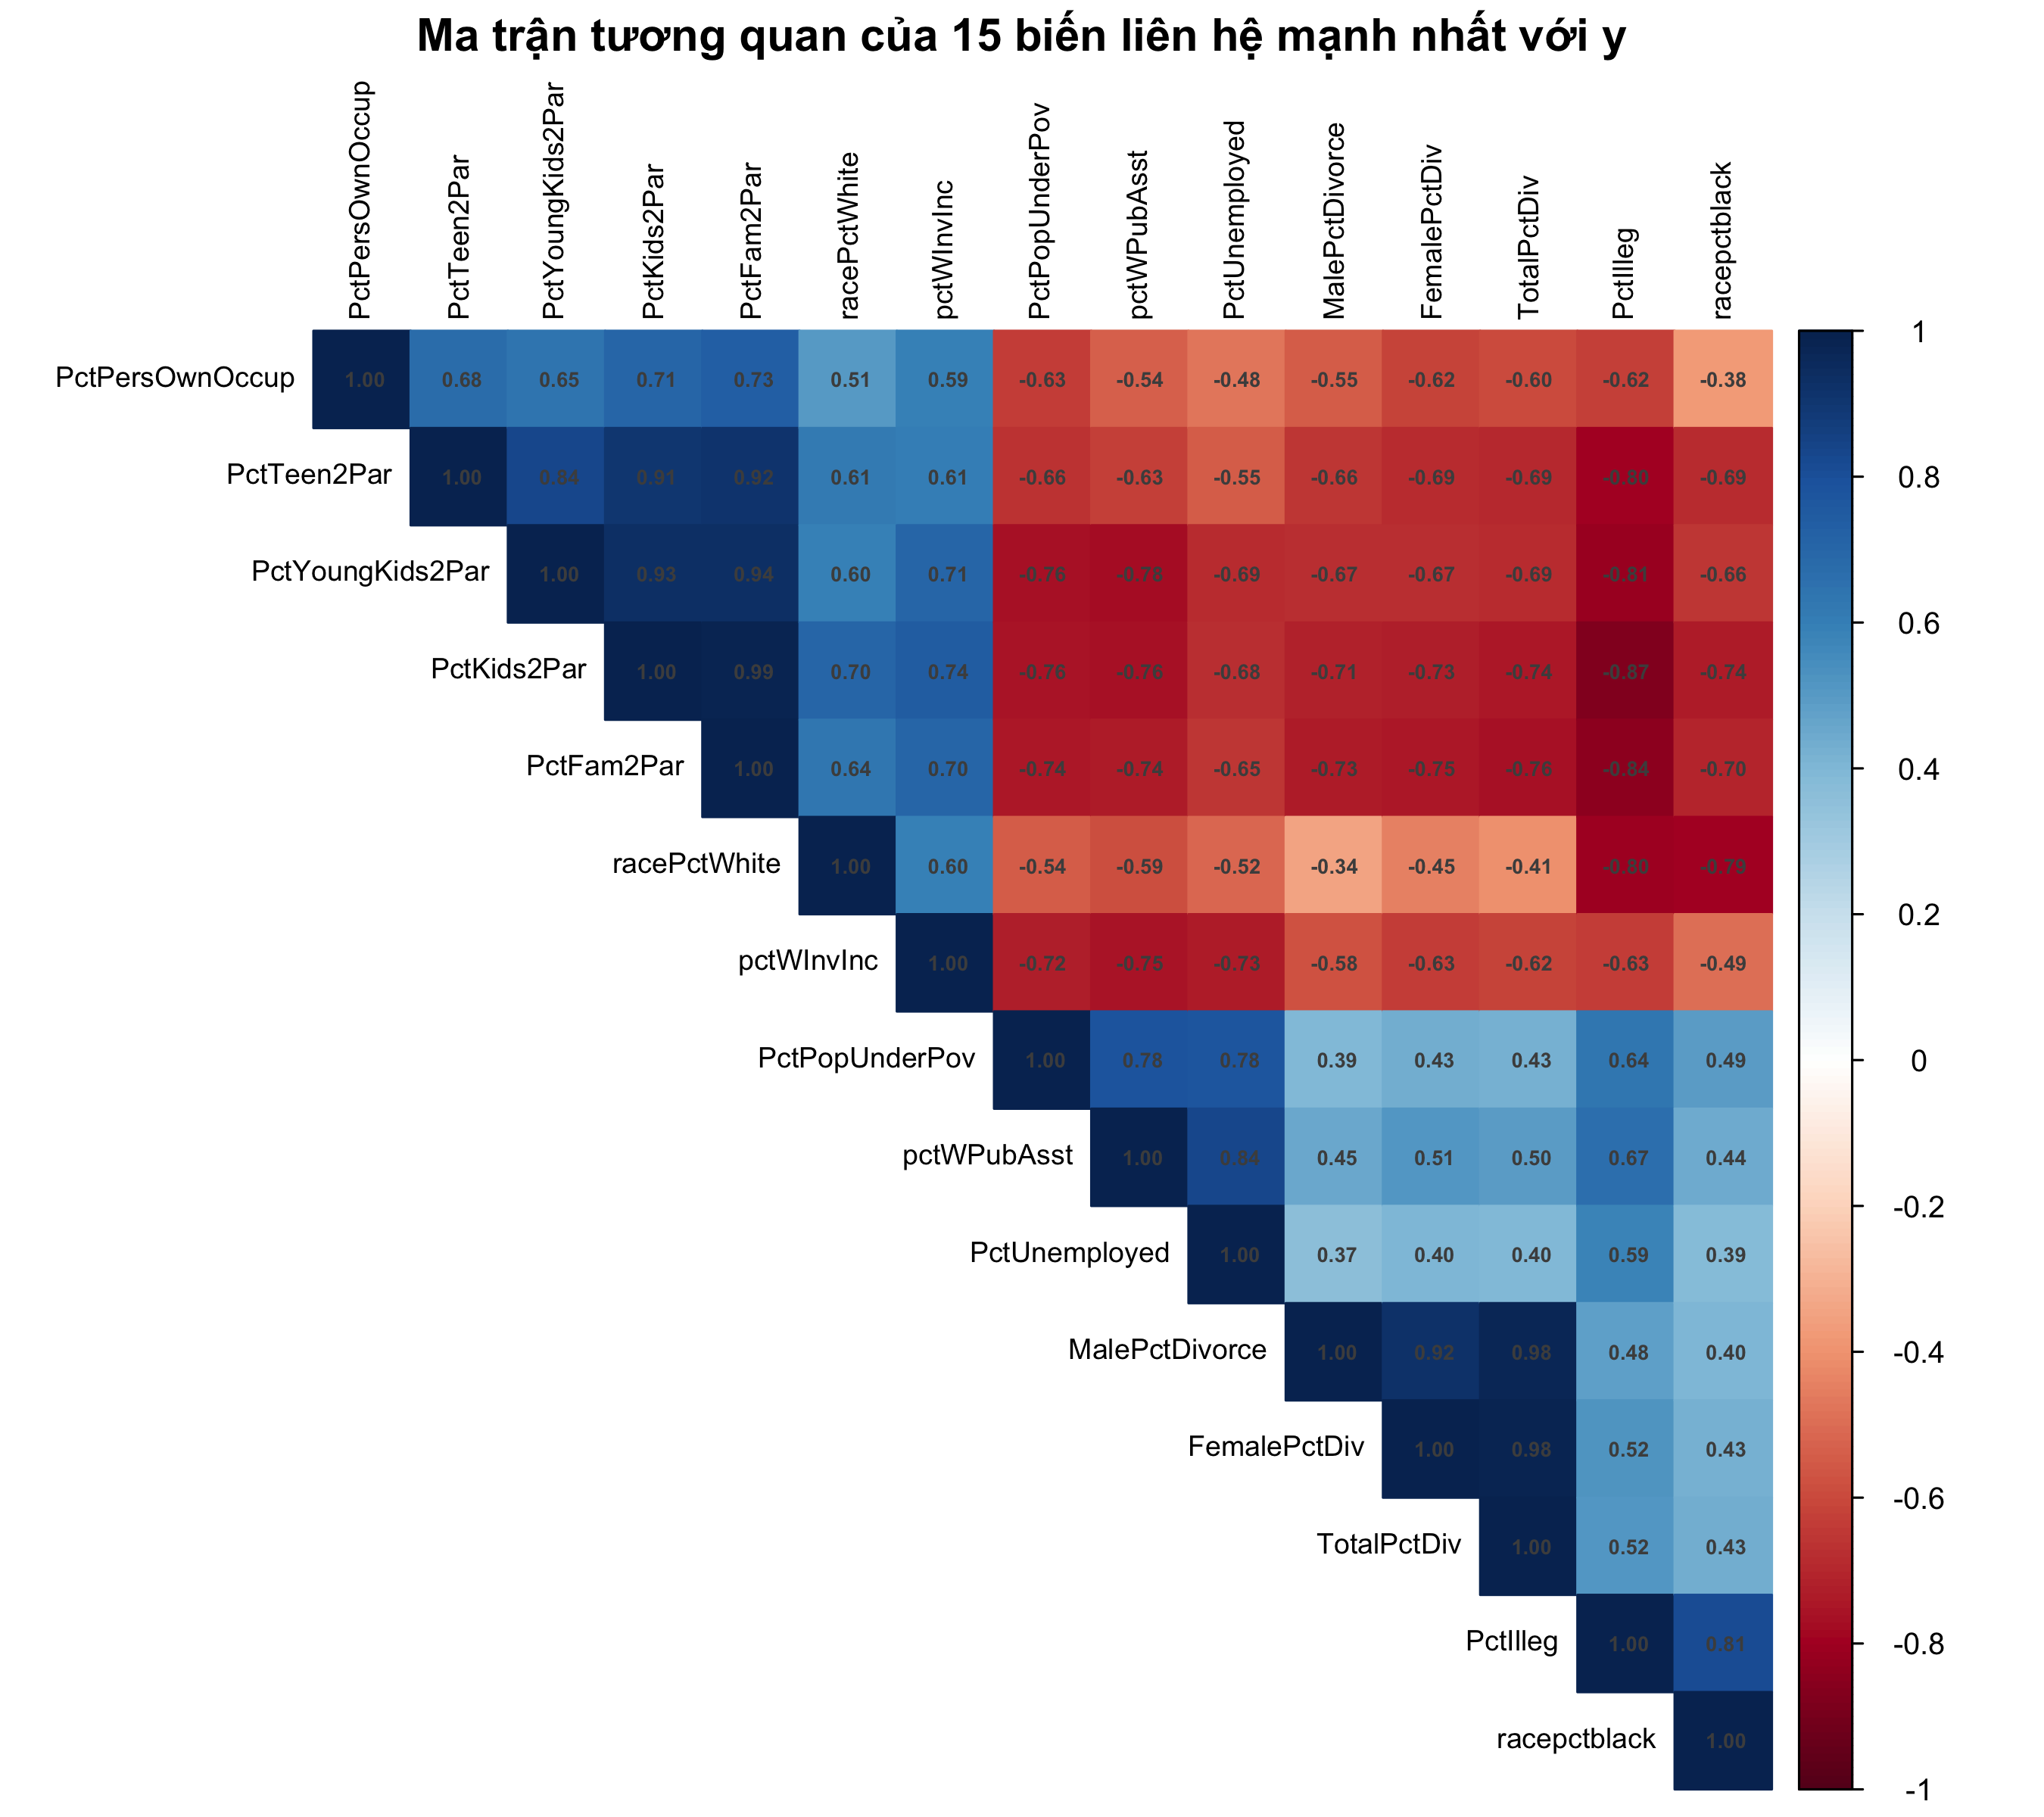
\includegraphics[width=\linewidth,keepaspectratio]{img/crime-cor-heatmap-1.png} \end{center}

\begin{longtable}[t]{lrl}
\caption{\label{tab:cor-heatmap}Số cặp biến dự báo có tương quan tuyệt đối vượt ngưỡng.}\\
\toprule
Ngưỡng & Số cặp biến & Trên tổng số cặp\\
\midrule
$\lvert r \rvert > 0.8$ & 127 & 4950\\
$\lvert r \rvert > 0.9$ & 49 & 4950\\
\bottomrule
\end{longtable}

\textbf{Nhận xét.} Hai điều nổi bật từ kết quả trên:

\begin{itemize}
\tightlist
\item
  \textbf{Về liên hệ với biến phản hồi:} các biến tương quan mạnh nhất
  với tỷ lệ tội phạm đều thuộc nhóm \textbf{cấu trúc gia đình}:
  \texttt{PctKids2Par} (\(r = -0.738\)), \texttt{PctIlleg}
  (\(r = 0.738\)), \texttt{PctFam2Par} (\(r = -0.707\)) và cùng các biến
  cơ cấu chủng tộc và nghèo đói (\texttt{racePctWhite},
  \texttt{pctWPubAsst}, \texttt{PctPopUnderPov}). Dấu của ma trận tương
  quan nhất quán với trực giác của chúng ta đối với xã hội: cộng đồng có
  tỷ lệ trẻ em sống cùng hai bố mẹ cao thì tỷ lệ tội phạm thấp, và ngược
  lại với tỷ lệ nghèo/trợ cấp.
\item
  \textbf{Về tương quan giữa các biến dự báo:} có tới 127 cặp biến với
  \(|r| > 0.8\) và 49 cặp với \(|r| > 0.9\) (tối đa \(|r| = 0.996\)).
  Ngay trong hình trên cũng thấy các khối biến gần như trùng thông tin
  (\texttt{PctFam2Par}, \texttt{PctKids2Par}, \texttt{PctYoungKids2Par},
  \texttt{PctTeen2Par}; \texttt{TotalPctDiv}, \texttt{FemalePctDiv},
  \texttt{MalePctDivorce}).
  Đây là biểu hiện trực tiếp của \textbf{đa cộng tuyến}, được định lượng
  chặt chẽ hơn ngay dưới đây.
\end{itemize}

\subsubsection{Chẩn đoán đa cộng tuyến định
lượng}\label{chux1ea9n-ux111ouxe1n-ux111a-cux1ed9ng-tuyux1ebfn-ux111ux1ecbnh-lux1b0ux1ee3ng}

Mức độ đa cộng tuyến được đo bằng hai công cụ như sau:

\begin{itemize}
\tightlist
\item
  \textbf{Chỉ số điều kiện (condition index)} của ma trận tương quan
  \(\mathbf{R} = \frac{1}{n-1}\mathbf{X}_s^\top \mathbf{X}_s\) (với
  \(\mathbf{X}_s\) đã chuẩn hóa):
  \(\kappa = \sqrt{\lambda_{\max} / \lambda_{\min}}\), trong đó
  \(\lambda_j\) là các trị riêng. Theo tiêu chuẩn Belsley, Kuh \& Welsch
  (1980), \(\kappa > 30\) là dấu hiệu đa cộng tuyến nghiêm trọng. Nếu ta
  xét theo ý nghĩa hình học: \(\lambda_{\min} \approx 0\) nghĩa là tồn
  tại một tổ hợp tuyến tính của các cột \(\mathbf{X}\) có phương sai gần
  bằng 0. Các cột gần phụ thuộc tuyến tính, khiến
  \((\mathbf{X}^\top\mathbf{X})^{-1}\) (và do đó phương sai của
  \(\hat{\beta}_{OLS}\)) bùng nổ.
\item
  \textbf{Hệ số phóng đại phương sai}
  \(\mathrm{VIF}_j = 1/(1 - R_j^2)\), với \(R_j^2\) là hệ số xác định
  khi hồi quy biến \(X_j\) trên toàn bộ các biến còn lại.
  \(\mathrm{VIF}_j > 10\) (tức \(R_j^2 > 0.9\)) là ngưỡng cảnh báo thông
  dụng; \(\mathrm{Var}(\hat\beta_j)\) tỷ lệ thuận với
  \(\mathrm{VIF}_j\).
\end{itemize}

\begin{longtable}[t]{lll}
\caption{\label{tab:da-cong-tuyen}Chẩn đoán đa cộng tuyến trên ma trận 100 biến dự báo.}\\
\toprule
Chỉ tiêu & Giá trị & Ngưỡng tham chiếu\\
\midrule
$\lambda_{\max}$ & 25.18 & —\\
$\lambda_{\min}$ & 0.00063 & —\\
Chỉ số điều kiện $\kappa = \sqrt{\lambda_{\max}/\lambda_{\min}}$ & 199.9 & > 30: nghiêm trọng (Belsley)\\
Số biến có VIF > 10 & 65 / 100 & VIF > 10: đáng lo ngại\\
Số biến có VIF > 100 & 22 & —\\
\addlinespace
VIF lớn nhất & 1037 & —\\
\bottomrule
\end{longtable}

\begin{longtable}[t]{lr}
\caption{\label{tab:da-cong-tuyen-vif}5 biến có VIF cao nhất.}\\
\toprule
Biến & VIF\\
\midrule
TotalPctDiv & 1037\\
OwnOccMedVal & 578\\
PctPersOwnOccup & 570\\
PctHousOwnOcc & 551\\
PctRecImmig8 & 478\\
\bottomrule
\end{longtable}

\textbf{Nhận xét.} Mọi chỉ tiêu đều vượt ngưỡng cảnh báo \textbf{rất
xa}: chỉ số điều kiện \(\kappa \approx 200\) gấp gần 7 lần ngưỡng
``nghiêm trọng'' 30 của Belsley. 65/100 biến có VIF \textgreater{} 10,
trong đó 22 biến có VIF \textgreater{} 100, cực đại là
\texttt{TotalPctDiv} với VIF \(\approx 1037\) (nghĩa là phương sai ước
lượng hệ số của biến này bị phóng đại hơn nghìn lần so với trường hợp
trực giao). Kết luận: \textbf{OLS trên toàn bộ biến sẽ cho các hệ số cực
kỳ bất ổn định}, dù khả năng dự đoán tổng thể có thể vẫn chấp nhận được.
Đây chính là bối cảnh mà các phương pháp \textbf{PCR, Ridge và LASSO}
được thiết kế để giải quyết bằng cách giảm chiều (PCR) hoặc chuẩn hóa
(Ridge/LASSO) nhằm đánh đổi một lượng chệch (bias) nhỏ lấy mức giảm
phương sai lớn.

\subsubsection{Giá trị ngoại lai}\label{giuxe1-trux1ecb-ngoux1ea1i-lai}

Cuối cùng, ta khảo sát giá trị ngoại lai bằng \textbf{phương pháp IQR}
của Tukey: giá trị bị xem là ngoại lai nếu nằm ngoài
\([Q_1 - 1.5\,\mathrm{IQR},\; Q_3 + 1.5\,\mathrm{IQR}]\). Ta chọn quy
tắc này để xác định các giá trị ngoại lai vì nó \textbf{không đặt giả
định phân phối}: hàng rào chỉ dựa trên các tứ phân vị do đó vẫn sẽ có ý
nghĩa với phân phối lệch, khác với quy tắc \(\bar{x} \pm 3s\) vốn chỉ
hợp lý dưới giả định dwx liệu tuân theo phân phối chuẩn.

\begin{longtable}[t]{ll}
\caption{\label{tab:outlier-iqr}Kết quả gắn cờ ngoại lai theo quy tắc IQR trên 100 biến dự báo.}\\
\toprule
Chỉ tiêu & Giá trị\\
\midrule
Tỷ lệ ô giá trị bị gắn cờ (toàn bảng) & 4.74 \%\\
Số quan sát có ít nhất 1 biến bị gắn cờ & 1538 / 1994 (77.1 \%)\\
Số quan sát bị gắn cờ ở từ 10 biến trở lên & 373\\
\bottomrule
\end{longtable}

\begin{center}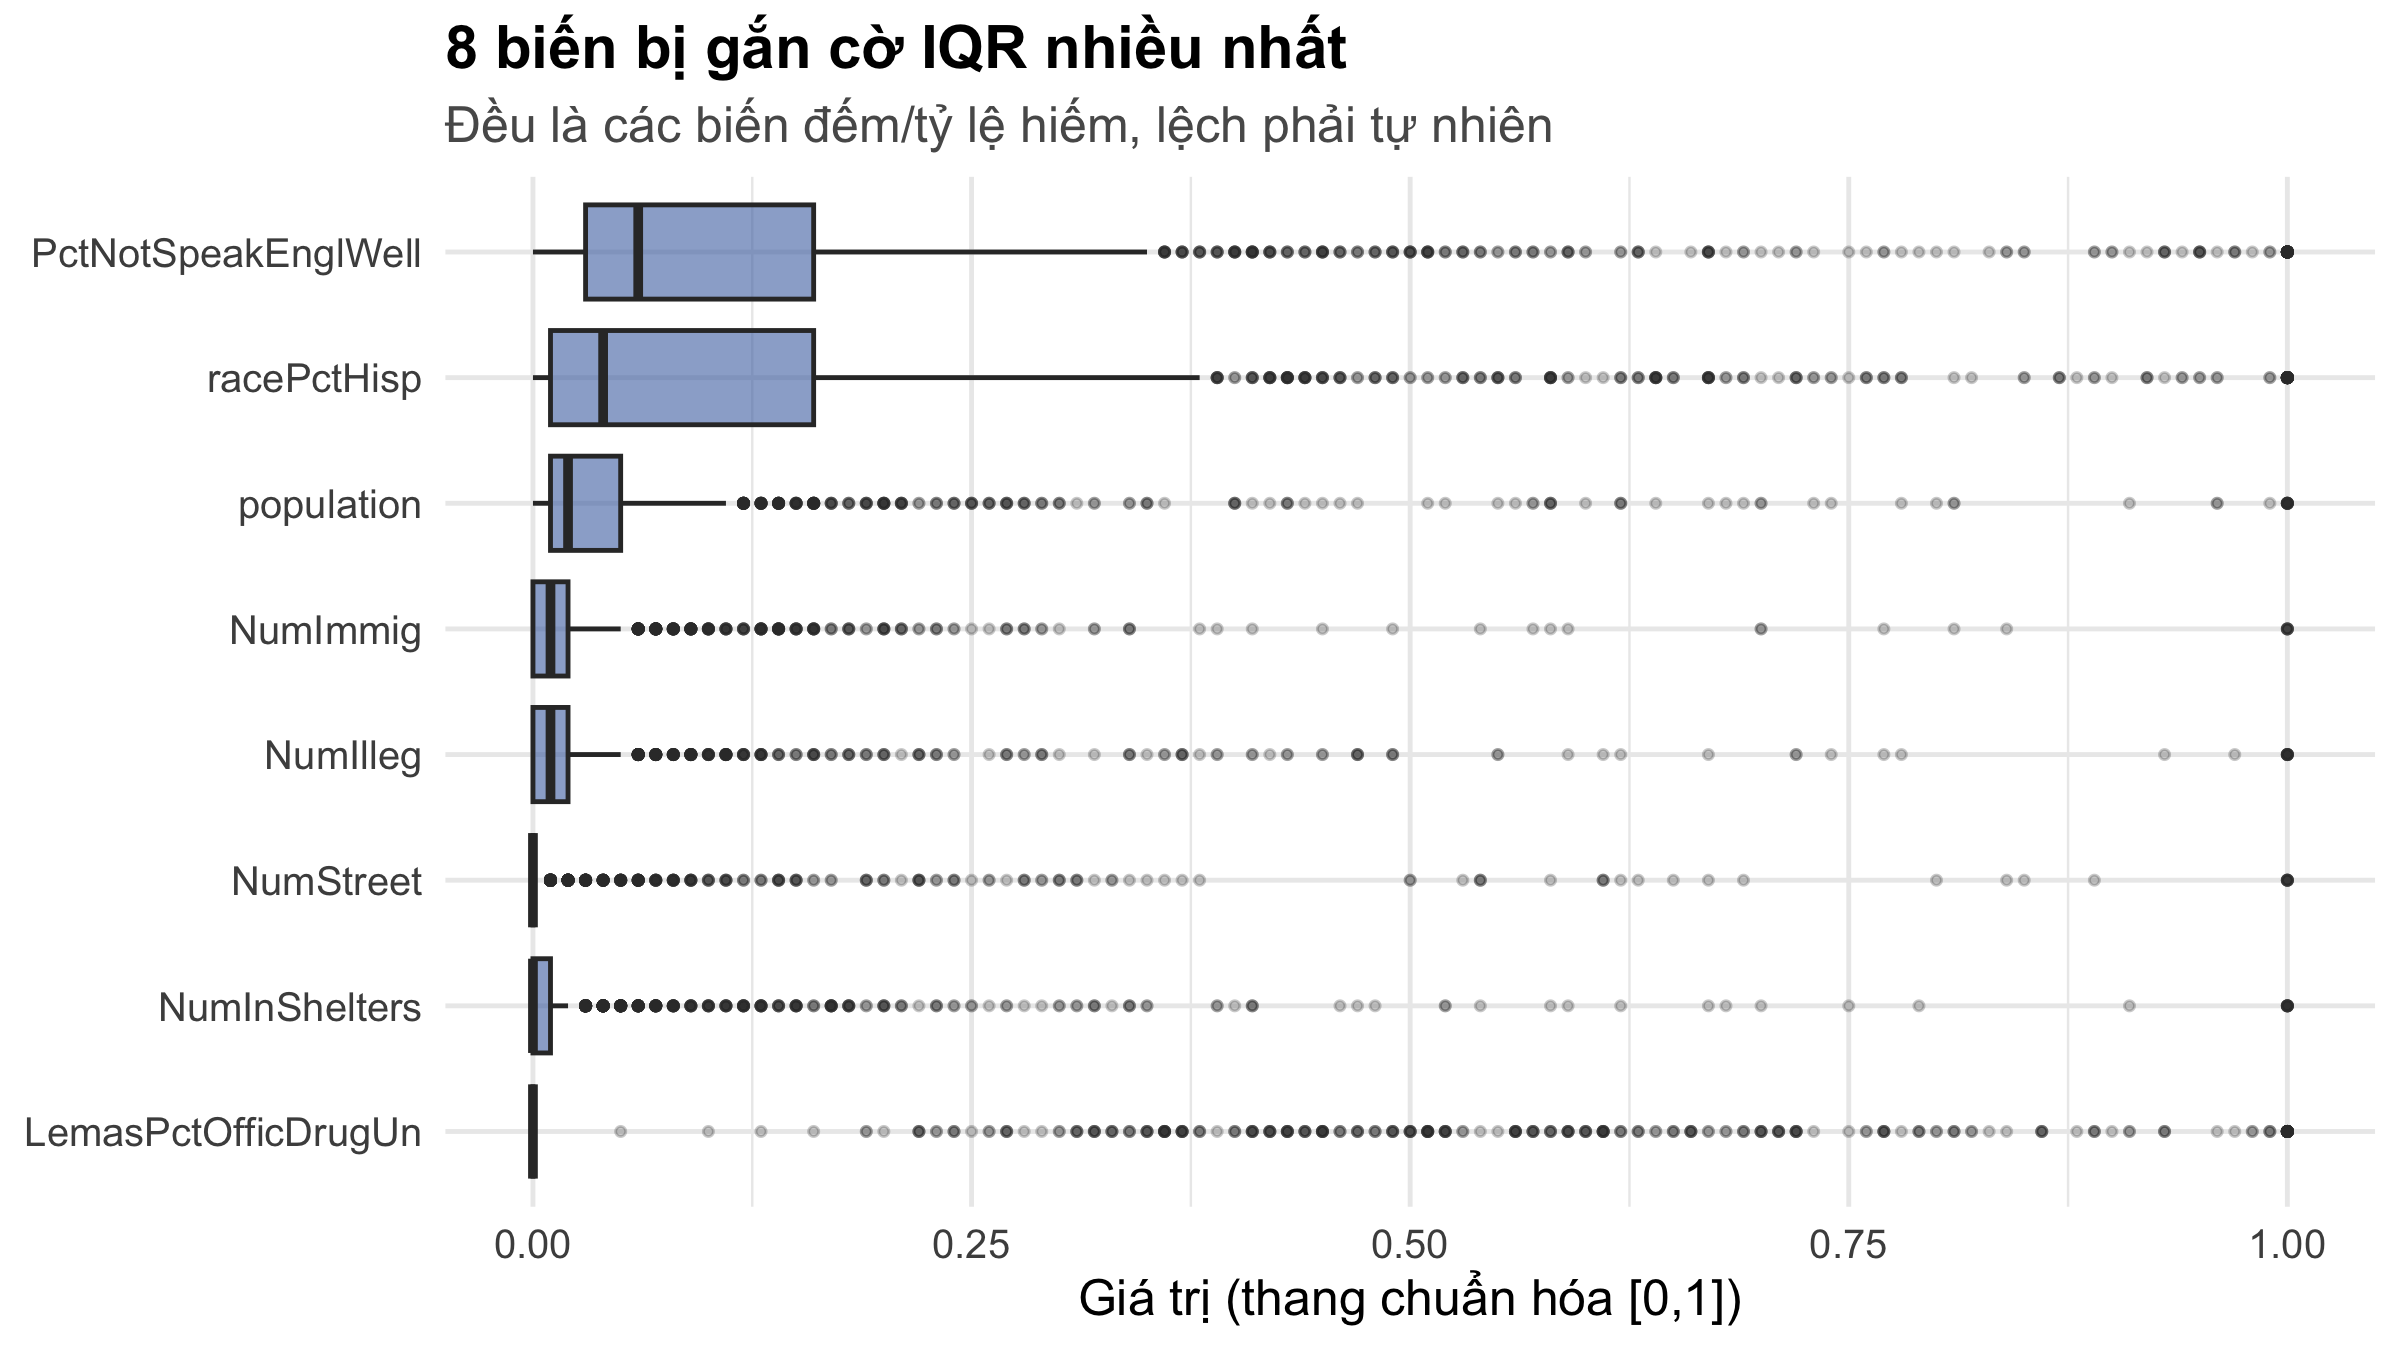
\includegraphics[width=\linewidth,keepaspectratio]{img/crime-outlier-iqr-1.png} \end{center}

\textbf{Nhận xét và quyết định.} Nếu loại mọi quan sát có ít nhất một
giá trị bị gắn cờ, ta sẽ mất 77.1\% dữ liệu và điều này tự nó cho thấy
``ngoại lai'' ở đây không phải lỗi đo lường mà là \textbf{đặc điểm cấu
trúc của dữ liệu}. Ta quyết định \textbf{không loại quan sát nào}, với
ba lý do:

\begin{enumerate}
\def\labelenumi{\arabic{enumi}.}
\tightlist
\item
  Các biến bị gắn cờ nhiều nhất (\texttt{NumStreet},
  \texttt{NumInShelters}, \texttt{NumIlleg}, \texttt{NumImmig}\ldots)
  đều là \textbf{biến đếm các hiện tượng hiếm}, phân phối lệch phải tự
  nhiên; giá trị lớn của chúng là thông tin thực (các thành phố lớn),
  không phải nhiễu.
\item
  Dữ liệu đã được tác giả \textbf{chuẩn hóa về thang \([0,1]\)}, trong
  đó giá trị lớn hơn 3 độ lệch chuẩn trên trung bình được gán bằng 1 và
  giá trị nhỏ hơn 3 độ lệch chuẩn dưới trung bình được gán bằng 0.
\item
  Các cộng đồng có tỷ lệ tội phạm cực cao chính là \textbf{đối tượng cần
  dự đoán}; loại chúng theo tiêu chí thống kê là tự cắt bỏ một phần miền
  giá trị của \(y\) (truncation có hệ thống), điều này làm chệch mô hình
  và giảm giá trị thực tiễn.
\end{enumerate}

\subsection{Tiền xử lý dữ
liệu}\label{tiux1ec1n-xux1eed-luxfd-dux1eef-liux1ec7u}

Từ các phát hiện của EDA, ta chốt các quyết định tiền xử lý sau.

\begin{longtable}[]{@{}
  >{\raggedright\arraybackslash}p{(\linewidth - 4\tabcolsep) * \real{0.1000}}
  >{\raggedright\arraybackslash}p{(\linewidth - 4\tabcolsep) * \real{0.3667}}
  >{\raggedright\arraybackslash}p{(\linewidth - 4\tabcolsep) * \real{0.5333}}@{}}
\toprule\noalign{}
\begin{minipage}[b]{\linewidth}\raggedright
\#
\end{minipage} & \begin{minipage}[b]{\linewidth}\raggedright
Quyết định
\end{minipage} & \begin{minipage}[b]{\linewidth}\raggedright
Lý do thống kê
\end{minipage} \\
\midrule\noalign{}
\endhead
\bottomrule\noalign{}
\endlastfoot
1 & \textbf{Bỏ 5 biến non-predictive} \texttt{state}, \texttt{county},
\texttt{community}, \texttt{communityname}, \texttt{fold} &
\texttt{state/county/community} là \textbf{mã danh nghĩa (nominal)}:
khoảng cách số học giữa hai mã không mang ý nghĩa, đưa vào hồi quy như
biến liên tục là sai bản chất thang đo; mã hóa one-hot sẽ tạo
\textasciitilde46 cột thưa, làm tăng chiều và nhiễu cấu trúc PCA.
\texttt{communityname} là chuỗi ký tự. \texttt{fold} là chỉ số kỹ thuật
do tác giả tạo, không phải đặc điểm của cộng đồng. \\
2 & \textbf{Bỏ 22 biến khối LEMAS khuyết 84\%} & Khuyết theo khối và
liên hệ rõ với quy mô cộng đồng. Imputation đòi hỏi ngoại suy cho phần
lớn mẫu; complete-case làm mất 1675/1994 quan sát và chỉ giữ các cộng
đồng lớn. \\
3 & \textbf{Điền khuyết \texttt{OtherPerCap} (1 giá trị) bằng trung vị
tập huấn luyện} & Trung vị là ước lượng vị trí \textbf{bền vững
(robust)}, không đặt giả định phân phối --- phù hợp vì các biến thu nhập
lệch phải. Với đúng 1/1994 giá trị khuyết, mọi phương pháp điền hợp lý
đều cho kết quả thực tế như nhau; ta chọn phương án đơn giản và không rò
rỉ thông tin. \\
4 & \textbf{Giữ nguyên tất cả quan sát} (không lọc ngoại lai) & Ba lý do
đã trình bày ở phần ngoại lai: cờ IQR phủ 77\% quan sát; dữ liệu nguồn
đã gán các giá trị ngoài khoảng 3 độ lệch chuẩn về 0 hoặc 1; loại quan
sát cực đoan của \(y\) là truncation làm chệch mô hình. \\
5 & \textbf{Kiểm tra biến phương sai gần 0} & Biến gần như hằng số không
mang thông tin nhưng có thể gây bất ổn số học khi chuẩn hóa (chia cho
\(s \approx 0\)) và khi nghịch đảo ma trận tương quan. \\
\end{longtable}

\begin{longtable}[t]{ll}
\caption{\label{tab:tien-xu-ly}Kiểm tra biến phương sai gần 0.}\\
\toprule
Chỉ tiêu & Kết quả\\
\midrule
Độ lệch chuẩn nhỏ nhất & 0.087\\
Biến tương ứng & NumImmig\\
Số biến có sd < 0.01 & 0\\
Số giá trị duy nhất ít nhất & 3 (biến MedNumBR)\\
\bottomrule
\end{longtable}

\textbf{Nhận xét.} Không có biến nào phương sai gần 0 (độ lệch chuẩn nhỏ
nhất 0.087 thuộc về \texttt{NumImmig} --- vẫn đủ lớn) do đó nên không
cần loại thêm biến nào ở bước này. Biến \texttt{MedNumBR} chỉ nhận 3 giá
trị phân biệt (do là trung vị số phòng ngủ đã chuẩn hóa) nhưng vẫn có
phương sai đáng kể nên được giữ lại. Sau tiền xử lý, ma trận biến dự báo
gồm \(n = 1994\) quan sát và \(p = 100\) biến và biến khuyết duy nhất
còn lại (\texttt{OtherPerCap}, 1 giá trị) sẽ được điền \textbf{sau khi
chia dữ liệu} để tuân thủ nguyên tắc chống rò rỉ thông tin.

\subsection{Chia dữ liệu}\label{chia-dux1eef-liux1ec7u}

\subsubsection{Nguyên tắc chống rò rỉ thông tin (data
leakage)}\label{nguyuxean-tux1eafc-chux1ed1ng-ruxf2-rux1ec9-thuxf4ng-tin-data-leakage}

Tập kiểm định (\emph{validation set}) có nhiệm vụ mô phỏng dữ liệu
\textbf{chưa từng thấy}. Vì vậy, mọi đại lượng ước lượng từ dữ liệu
trong quá trình tiền xử lý và huấn luyện và những thứ như trung vị điền
khuyết, trung bình \(\bar{x}_j\) và độ lệch chuẩn \(s_j\) dùng để chuẩn
hóa, các vector tải của PCA, tham số \(\lambda\) của Ridge/LASSO sẽ đều
chỉ được \textbf{ước lượng trên tập huấn luyện}, sau đó \textbf{áp
nguyên} sang tập kiểm định. Nếu vi phạm (ví dụ chuẩn hóa trên toàn bộ dữ
liệu trước khi chia), thông tin của tập kiểm định sẽ ``rò'' vào mô hình,
khiến các chỉ số đánh giá lạc quan hơn thực tế một cách hệ thống và
không có tính ứng dụng cao cho dữ liệu mới mà không có trong tập huấn
luyện.

\subsubsection{Thực hiện chia và kiểm tra phân
phối}\label{thux1ef1c-hiux1ec7n-chia-vuxe0-kiux1ec3m-tra-phuxe2n-phux1ed1i}

Ta chia ngẫu nhiên dữ liệu thành \textbf{80\% huấn luyện / 20\% kiểm
định}, tương ứng khoảng 1 595 quan sát huấn luyện và 399 quan sát kiểm
định. Kích thước tập huấn luyện lớn hơn nhiều so với số biến dự báo,
nhưng hiện tượng đa cộng tuyến vẫn có thể làm OLS bất ổn. So sánh thống
kê mô tả dưới đây chỉ nhằm kiểm tra xem lần chia có mất cân bằng rõ rệt
hay không, không phải bằng chứng chứng minh hai tập có phân phối hoàn
toàn giống nhau.

\begin{verbatim}
## n_train   n_val 
##    1595     399
\end{verbatim}

\begin{longtable}[t]{lrrrr}
\caption{\label{tab:kiem-tra-can-bang}So sánh phân phối biến phản hồi giữa hai tập.}\\
\toprule
Tập & n & Trung bình y & Trung vị y & Độ lệch chuẩn y\\
\midrule
Huấn luyện & 1595 & 0.234 & 0.15 & 0.230\\
Kiểm định & 399 & 0.252 & 0.17 & 0.244\\
\bottomrule
\end{longtable}

\textbf{Nhận xét.} Phép chia tạo \(n_{train} = 1595\) và
\(n_{val} = 399\). Trung bình, trung vị và độ lệch chuẩn của \(y\) gần
nhau giữa hai tập, nên lần chia không cho thấy mất cân bằng đáng kể. Giá
trị khuyết duy nhất của \texttt{OtherPerCap} được điền bằng trung vị học
trên tập huấn luyện (\(0.26\)).

\subsection{Mô hình hồi quy trên thành phần chính
(PCR)}\label{muxf4-huxecnh-hux1ed3i-quy-truxean-thuxe0nh-phux1ea7n-chuxednh-pcr}

\subsubsection{Cơ sở toán học}\label{cux1a1-sux1edf-touxe1n-hux1ecdc}

PCR xử lý đa cộng tuyến bằng cách thay 100 biến gốc bằng các
\textbf{thành phần chính}: những tổ hợp tuyến tính trực giao, được sắp
theo lượng phương sai của \(\mathbf X\) mà chúng giữ lại. Sau khi chuẩn
hóa dữ liệu huấn luyện, PCA phân rã ma trận tương quan thành

\[
\mathbf R = \mathbf V\boldsymbol{\Lambda}\mathbf V^\top,
\]

trong đó các cột của \(\mathbf V\) là hướng thành phần chính và
\(\lambda_j\) cho biết phương sai của thành phần thứ \(j\). PCR giữ
\(k\) hướng đầu, tạo \(\mathbf Z_k = \mathbf X_s\mathbf V_k\), rồi hồi
quy \(y\) trên \(\mathbf Z_k\).

Ý tưởng thống kê rất đơn giản: OLS dùng toàn bộ các hướng, kể cả những
hướng có phương sai rất nhỏ và dễ khuếch đại nhiễu. PCR bỏ các hướng sau
\(k\), chấp nhận mất một phần tín hiệu để giảm phương sai ước lượng. Vì
vậy, lựa chọn \(k\) phải dựa trên kiểm chứng chéo, không chỉ dựa trên tỷ
lệ phương sai của \(\mathbf X\).

Trong báo cáo này, PCA được thực hiện trên dữ liệu đã chuẩn hóa bằng
trung bình và độ lệch chuẩn học từ tập huấn luyện; cùng tham số đó được
áp sang tập kiểm định để tránh rò rỉ dữ liệu.

\subsubsection{Kiểm tra mức độ phù hợp của dữ liệu với
PCR}\label{kiux1ec3m-tra-mux1ee9c-ux111ux1ed9-phuxf9-hux1ee3p-cux1ee7a-dux1eef-liux1ec7u-vux1edbi-pcr}

Bartlett và KMO được dùng như chẩn đoán mô tả: chúng cho biết các biến
dự báo có tương quan đủ mạnh để PCA có ý nghĩa hay không. Hai kiểm tra
này chỉ nhìn vào \(\mathbf X\), nên không thay thế cho đánh giá dự đoán
bằng validation.

\begin{longtable}[t]{lll}
\caption{\label{tab:pcr-suitability}Kiểm tra mức độ phù hợp của dữ liệu với PCA/PCR (trên tập huấn luyện).}\\
\toprule
Chỉ tiêu & Giá trị & Diễn giải\\
\midrule
Bartlett $\chi^2$ & 342 736 & Rất lớn so với df\\
Bậc tự do & 4950 & $p(p-1)/2 = 4950$\\
p-value & < 1e-300 & Bác bỏ $H_0: R = I$\\
KMO tổng thể & 0.924 & Mức “tuyệt vời” ($\ge 0.9$)\\
KMO nhỏ nhất theo biến & 0.761 (PctEmplManu) & Vẫn trên mức chấp nhận 0.5\\
\addlinespace
Số biến có $MSA_i < 0.5$ & 0 & —\\
\bottomrule
\end{longtable}

\textbf{Nhận xét.} Bartlett bác bỏ giả thuyết ma trận tương quan đơn vị
(\(p < 10^{-300}\)), còn KMO tổng thể đạt \(0.924\). Dữ liệu vì vậy phù
hợp để giảm chiều bằng PCA, nhưng chất lượng dự đoán của PCR vẫn phải
được quyết định bằng kiểm chứng chéo.

\subsubsection{Phân tích thành phần chính trên tập huấn
luyện}\label{phuxe2n-tuxedch-thuxe0nh-phux1ea7n-chuxednh-truxean-tux1eadp-huux1ea5n-luyux1ec7n}

\begin{center}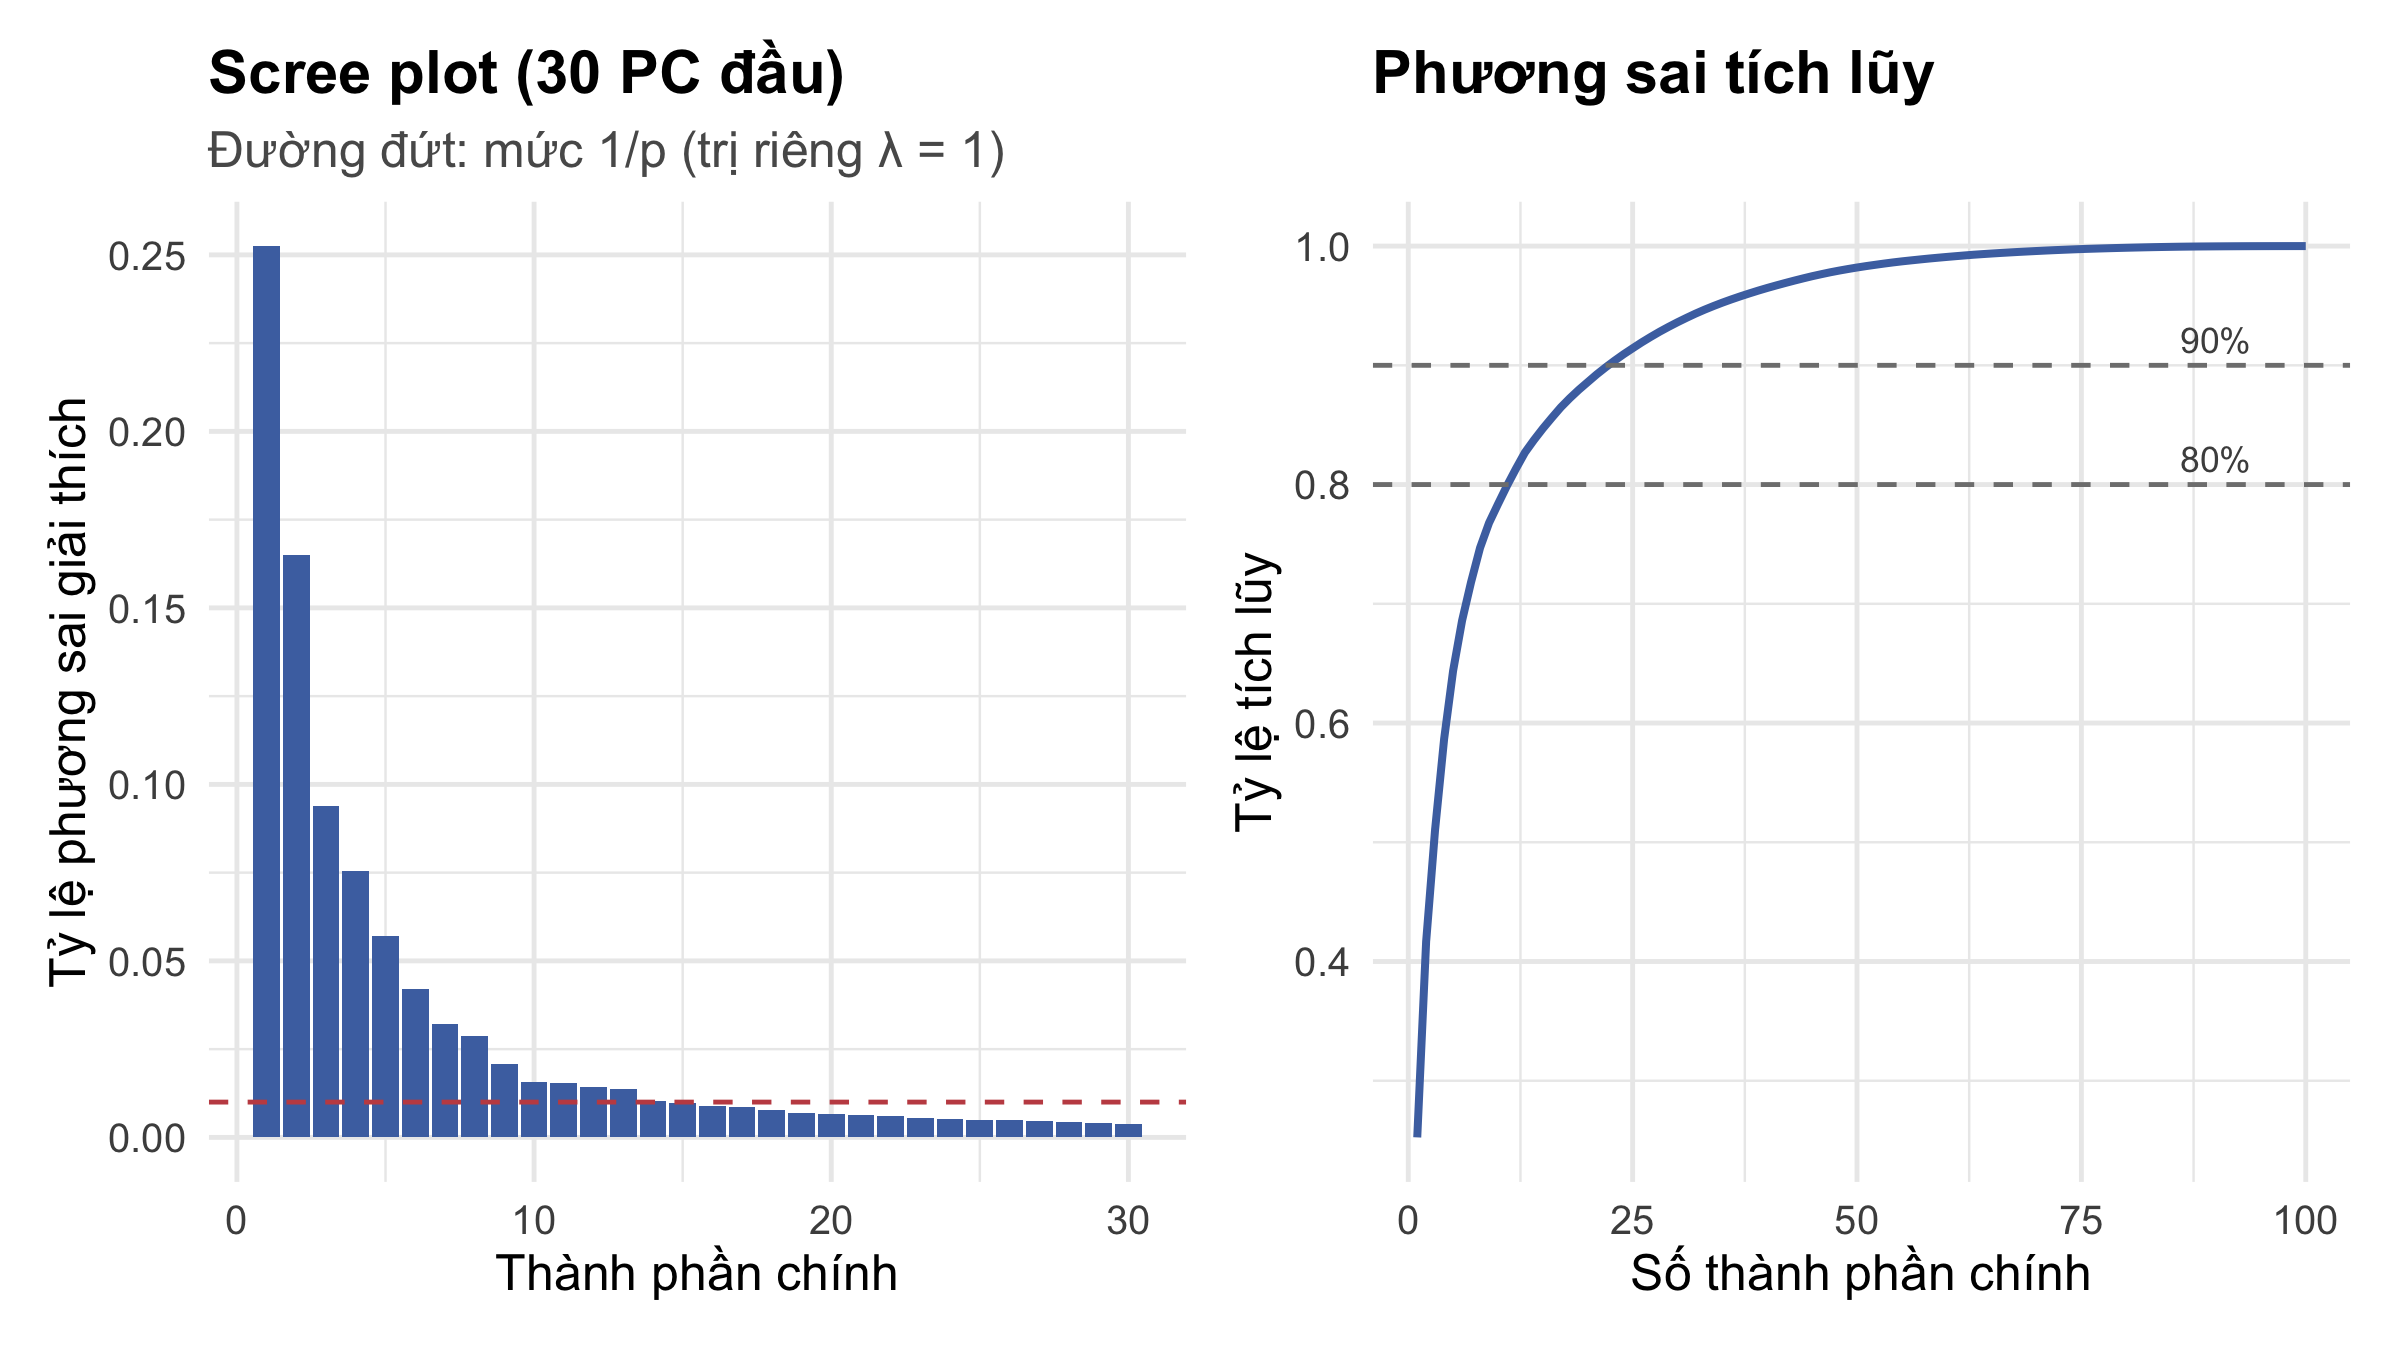
\includegraphics[width=\linewidth,keepaspectratio]{img/crime-pca-train-1.png} \end{center}

\begin{longtable}[t]{ll}
\caption{\label{tab:pca-train}Các tiêu chí mô tả về số thành phần chính.}\\
\toprule
Tiêu chí & Kết quả\\
\midrule
Kaiser: số PC có $\lambda_j > 1$ & 14\\
Số PC đạt 80\% phương sai tích lũy & 12\\
Số PC đạt 90\% phương sai tích lũy & 23\\
PVE của PC1 & 25.2 \%\\
PVE của PC2 & 16.5 \%\\
\bottomrule
\end{longtable}

\textbf{Nhận xét.} Cấu trúc nén thông tin rất rõ: chỉ riêng PC1 đã giải
thích 25.2\% tổng phương sai của 100 biến, hai thành phần đầu giải thích
41.7\%, và chỉ cần 12 thành phần để đạt 80\% (so với 100 chiều gốc).
Tiêu chí Kaiser (\(\lambda_j > 1\): thành phần ``mang nhiều thông tin
hơn một biến gốc đơn lẻ'') giữ 14 thành phần. Tuy nhiên các tiêu chí này
đều \textbf{chỉ nhìn vào \(\mathbf{X}\)} mà không nhìn vào \(y\) bởi
chúng đo lượng phương sai được giữ, không đo khả năng dự đoán. Quyết
định cuối cùng vì vậy dựa trên kiểm chứng chéo dưới đây.

\subsubsection{Lựa chọn số thành phần chính bằng kiểm chứng
chéo}\label{lux1ef1a-chux1ecdn-sux1ed1-thuxe0nh-phux1ea7n-chuxednh-bux1eb1ng-kiux1ec3m-chux1ee9ng-chuxe9o}

Ta chạy PCR với đủ 100 thành phần và kiểm chứng chéo 10-fold trên tập
huấn luyện. Quy tắc \textbf{one-sigma} giúp chọn mô hình đơn giản nhất
có sai số CV còn nằm trong vùng một độ lệch chuẩn quanh mô hình tốt
nhất. Ta đối chiếu thêm kiểm định hoán vị.

\begin{center}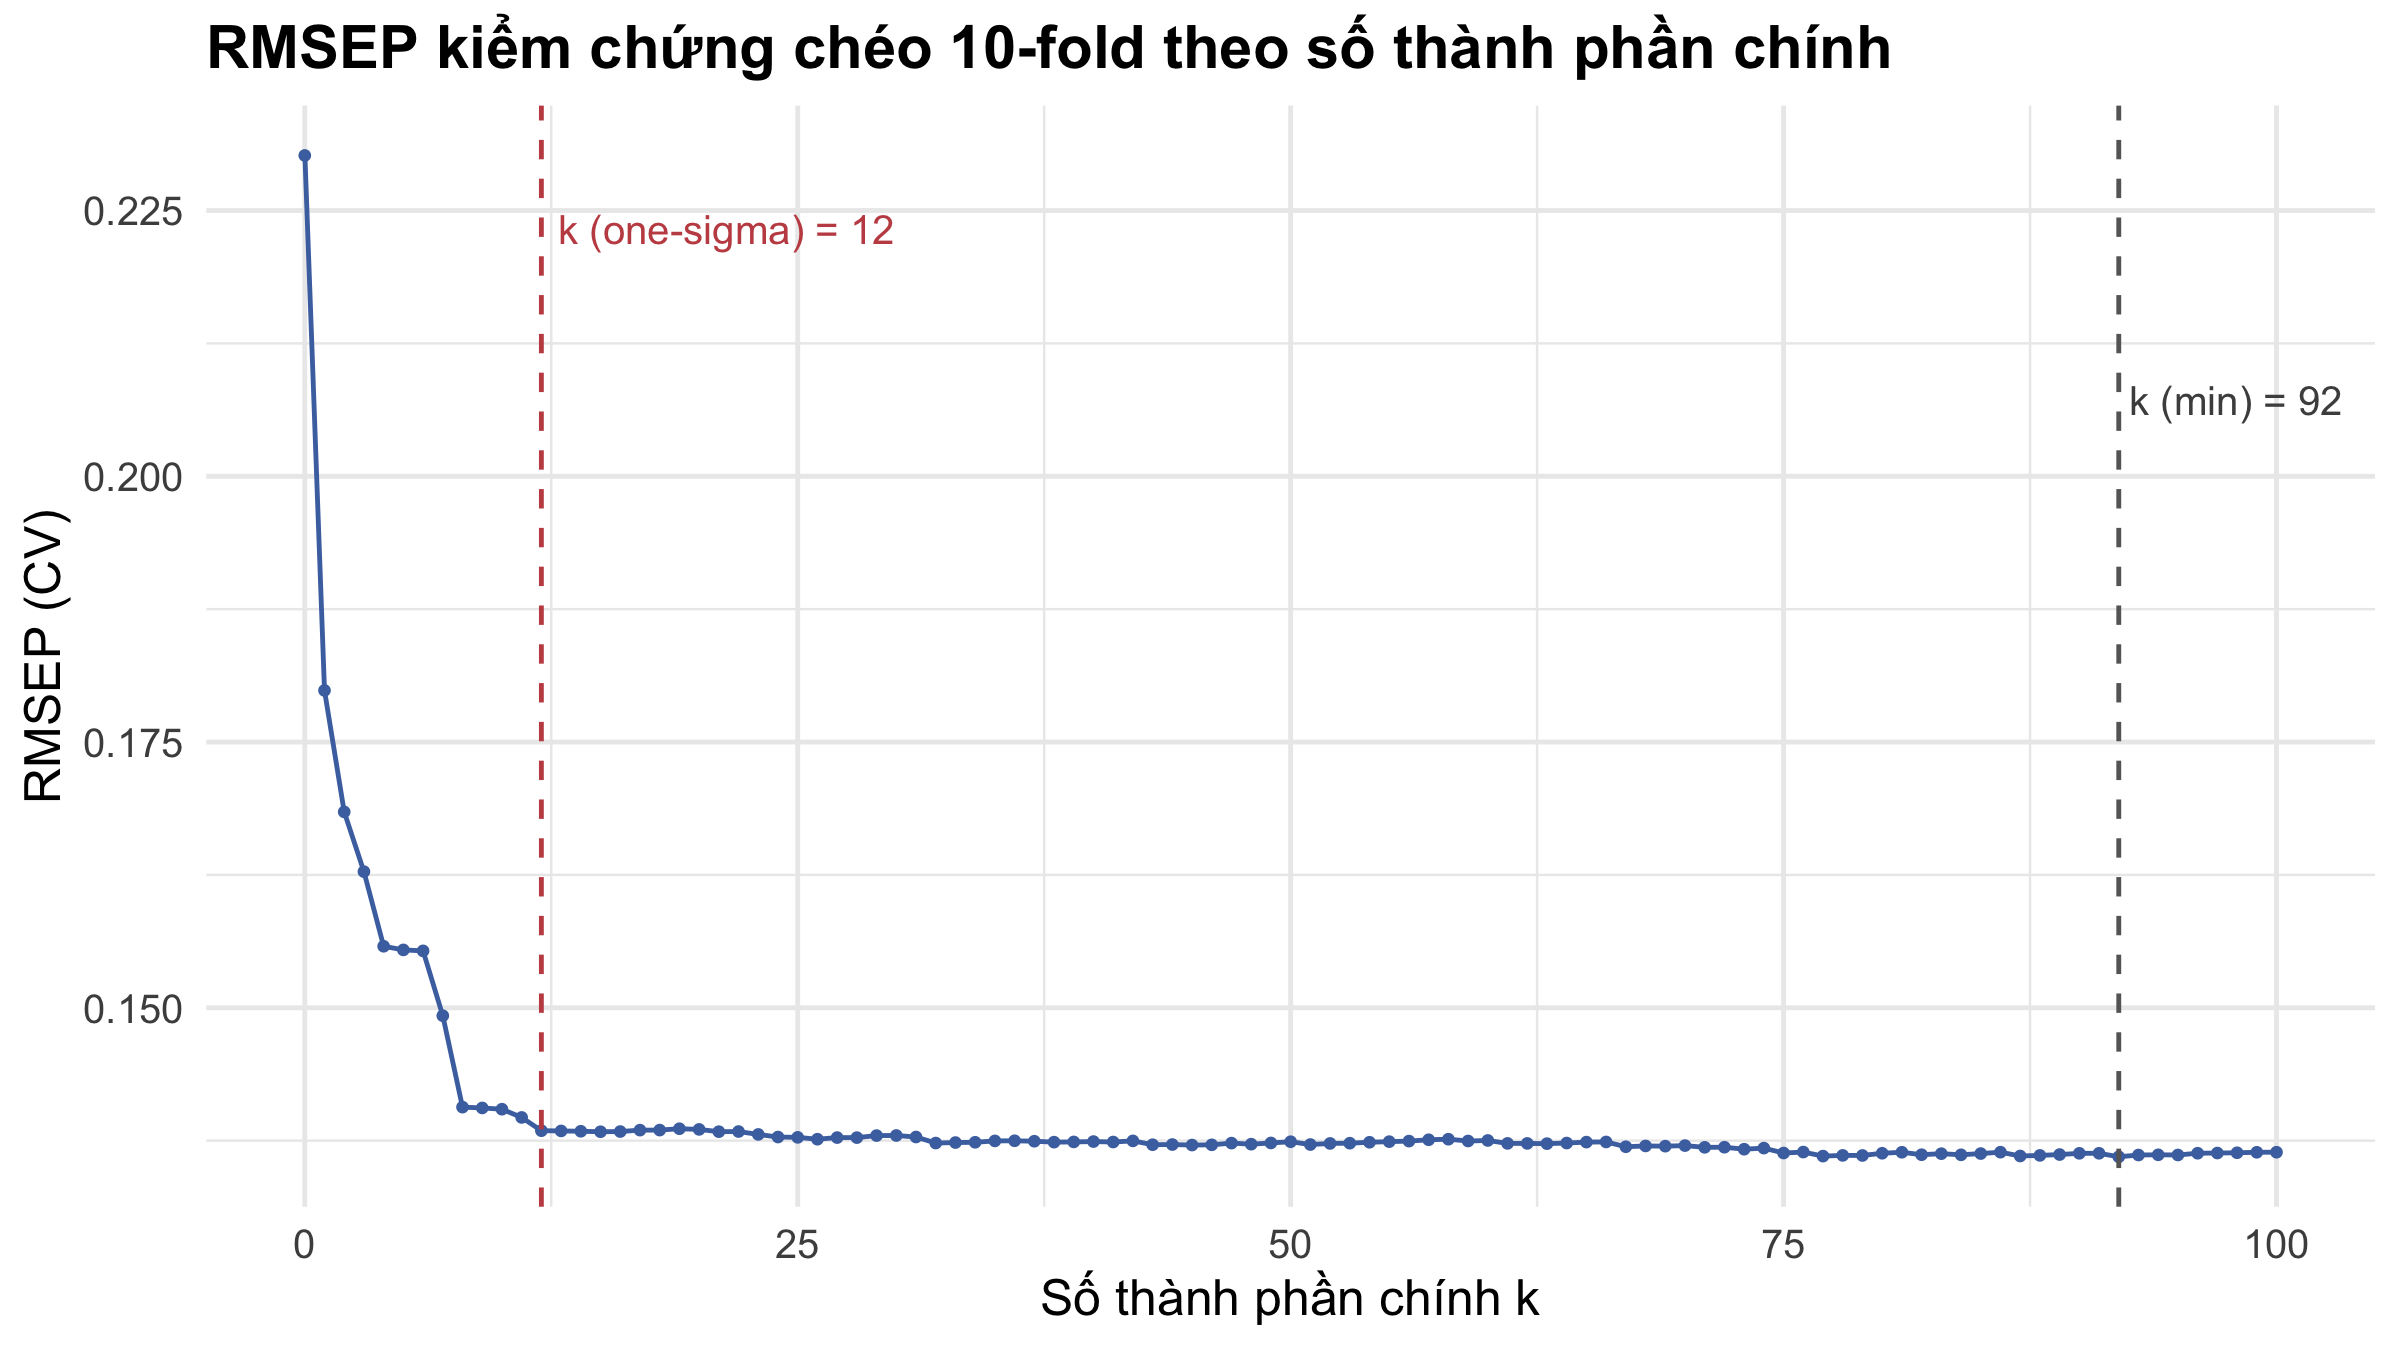
\includegraphics[width=\linewidth,keepaspectratio]{img/crime-pcr-cv-1.png} \end{center}

\begin{longtable}[t]{lrr}
\caption{\label{tab:pcr-cv}Số thành phần chính theo các quy tắc chọn trên CV.}\\
\toprule
Quy tắc & k & RMSEP (CV)\\
\midrule
Cực tiểu RMSEP & 92 & 0.1360\\
One-sigma & 12 & 0.1384\\
Randomization (van der Voet) & 12 & 0.1384\\
\bottomrule
\end{longtable}

\textbf{Nhận xét và quyết định.} Cực tiểu RMSEP nằm tại \(k = 92\), còn
one-sigma chọn \(k = 12\) với RMSEP cao hơn 0.0025. Ta chọn mô hình
one-sigma vì gọn hơn trong khi sai số CV gần cực tiểu; lựa chọn này giữ
81.3\% phương sai của \(\mathbf X\) và giảm số hệ số thành phần từ 100
xuống 12.

Mô hình PCR cuối cùng được huấn luyện với \(k = 12\) trên toàn bộ tập
huấn luyện; dự đoán trên tập kiểm định sẽ được đánh giá cùng các mô hình
đối chứng ở phần đánh giá.

\subsection{Các mô hình đối
chứng}\label{cuxe1c-muxf4-huxecnh-ux111ux1ed1i-chux1ee9ng}

\subsubsection{Hồi quy bình phương tối thiểu
(OLS)}\label{hux1ed3i-quy-buxecnh-phux1b0ux1a1ng-tux1ed1i-thiux1ec3u-ols}

Mô hình tuyến tính đặt
\(E(y_i\mid\mathbf x_i)=\beta_0+\mathbf x_i^\top\boldsymbol\beta\). Với
ma trận thiết kế mở rộng \(\widetilde{\mathbf X}=[\mathbf 1,\mathbf X]\)
và giả sử ma trận này có hạng đầy đủ,

\[
\hat{\boldsymbol\theta}_{OLS}
=\arg\min_{\boldsymbol\theta}\|\mathbf y-\widetilde{\mathbf X}\boldsymbol\theta\|_2^2
=(\widetilde{\mathbf X}^{\top}\widetilde{\mathbf X})^{-1}
\widetilde{\mathbf X}^{\top}\mathbf y,
\qquad \boldsymbol\theta=(\beta_0,\boldsymbol\beta^\top)^\top.
\]

Điều kiện \(E(\varepsilon\mid X)=0\) quyết định tính không chệch của
OLS. Nếu thêm giả định phương sai đồng nhất và không có tương quan giữa
các sai số, OLS là BLUE và công thức sai số chuẩn cổ điển là hợp lệ. Với
hệ số dốc thứ \(j\), ta có
\(\mathrm{Var}(\hat\beta_j)=\sigma^2\mathrm{VIF}_j/[(n-1)s_j^2]\), nên
đa cộng tuyến làm sai số chuẩn tăng và khiến suy diễn từng hệ số kém ổn
định, dù dự đoán tổng hợp vẫn có thể tốt.

\begin{longtable}[t]{lr}
\caption{\label{tab:ols-fit}Tóm tắt mô hình OLS đầy đủ trên tập huấn luyện.}\\
\toprule
Chỉ tiêu & Giá trị\\
\midrule
$R^2$ (huấn luyện) & 0.694\\
$R^2$ hiệu chỉnh & 0.673\\
Số biến dự báo có $|t| > 2$ & 24.000\\
Tổng số biến dự báo & 100.000\\
\bottomrule
\end{longtable}

\textbf{Nhận xét.} Mô hình giải thích được \(R^2 = 0.694\) phương sai
trên tập huấn luyện, nhưng chỉ 24/100 biến dự báo có \(|t| > 2\). Nghịch
lý ``mô hình khớp tốt nhưng hầu hết hệ số không có ý nghĩa'' là
\textbf{triệu chứng kinh điển của đa cộng tuyến}: thông tin chung bị
chia sẻ giữa các biến tương quan khiến từng hệ số riêng lẻ có sai số
chuẩn khổng lồ, đúng như dự báo từ các VIF ở phần đa cộng tuyến.

\paragraph{Chẩn đoán mô hình
OLS}\label{chux1ea9n-ux111ouxe1n-muxf4-huxecnh-ols}

Các biểu đồ và kiểm định sau được dùng để xem xét dạng tuyến tính,
phương sai phần dư, phân phối phần dư và các quan sát ảnh hưởng. Độc lập
giữa các cộng đồng và \(E(\varepsilon\mid X)=0\) là giả định thiết kế,
không thể xác nhận chỉ bằng đồ thị phần dư; vì vậy diễn giải hệ số vẫn
là liên hệ, không phải nhân quả. Khi phương sai không đồng nhất, ta dùng
thêm sai số chuẩn HC3.

\begin{center}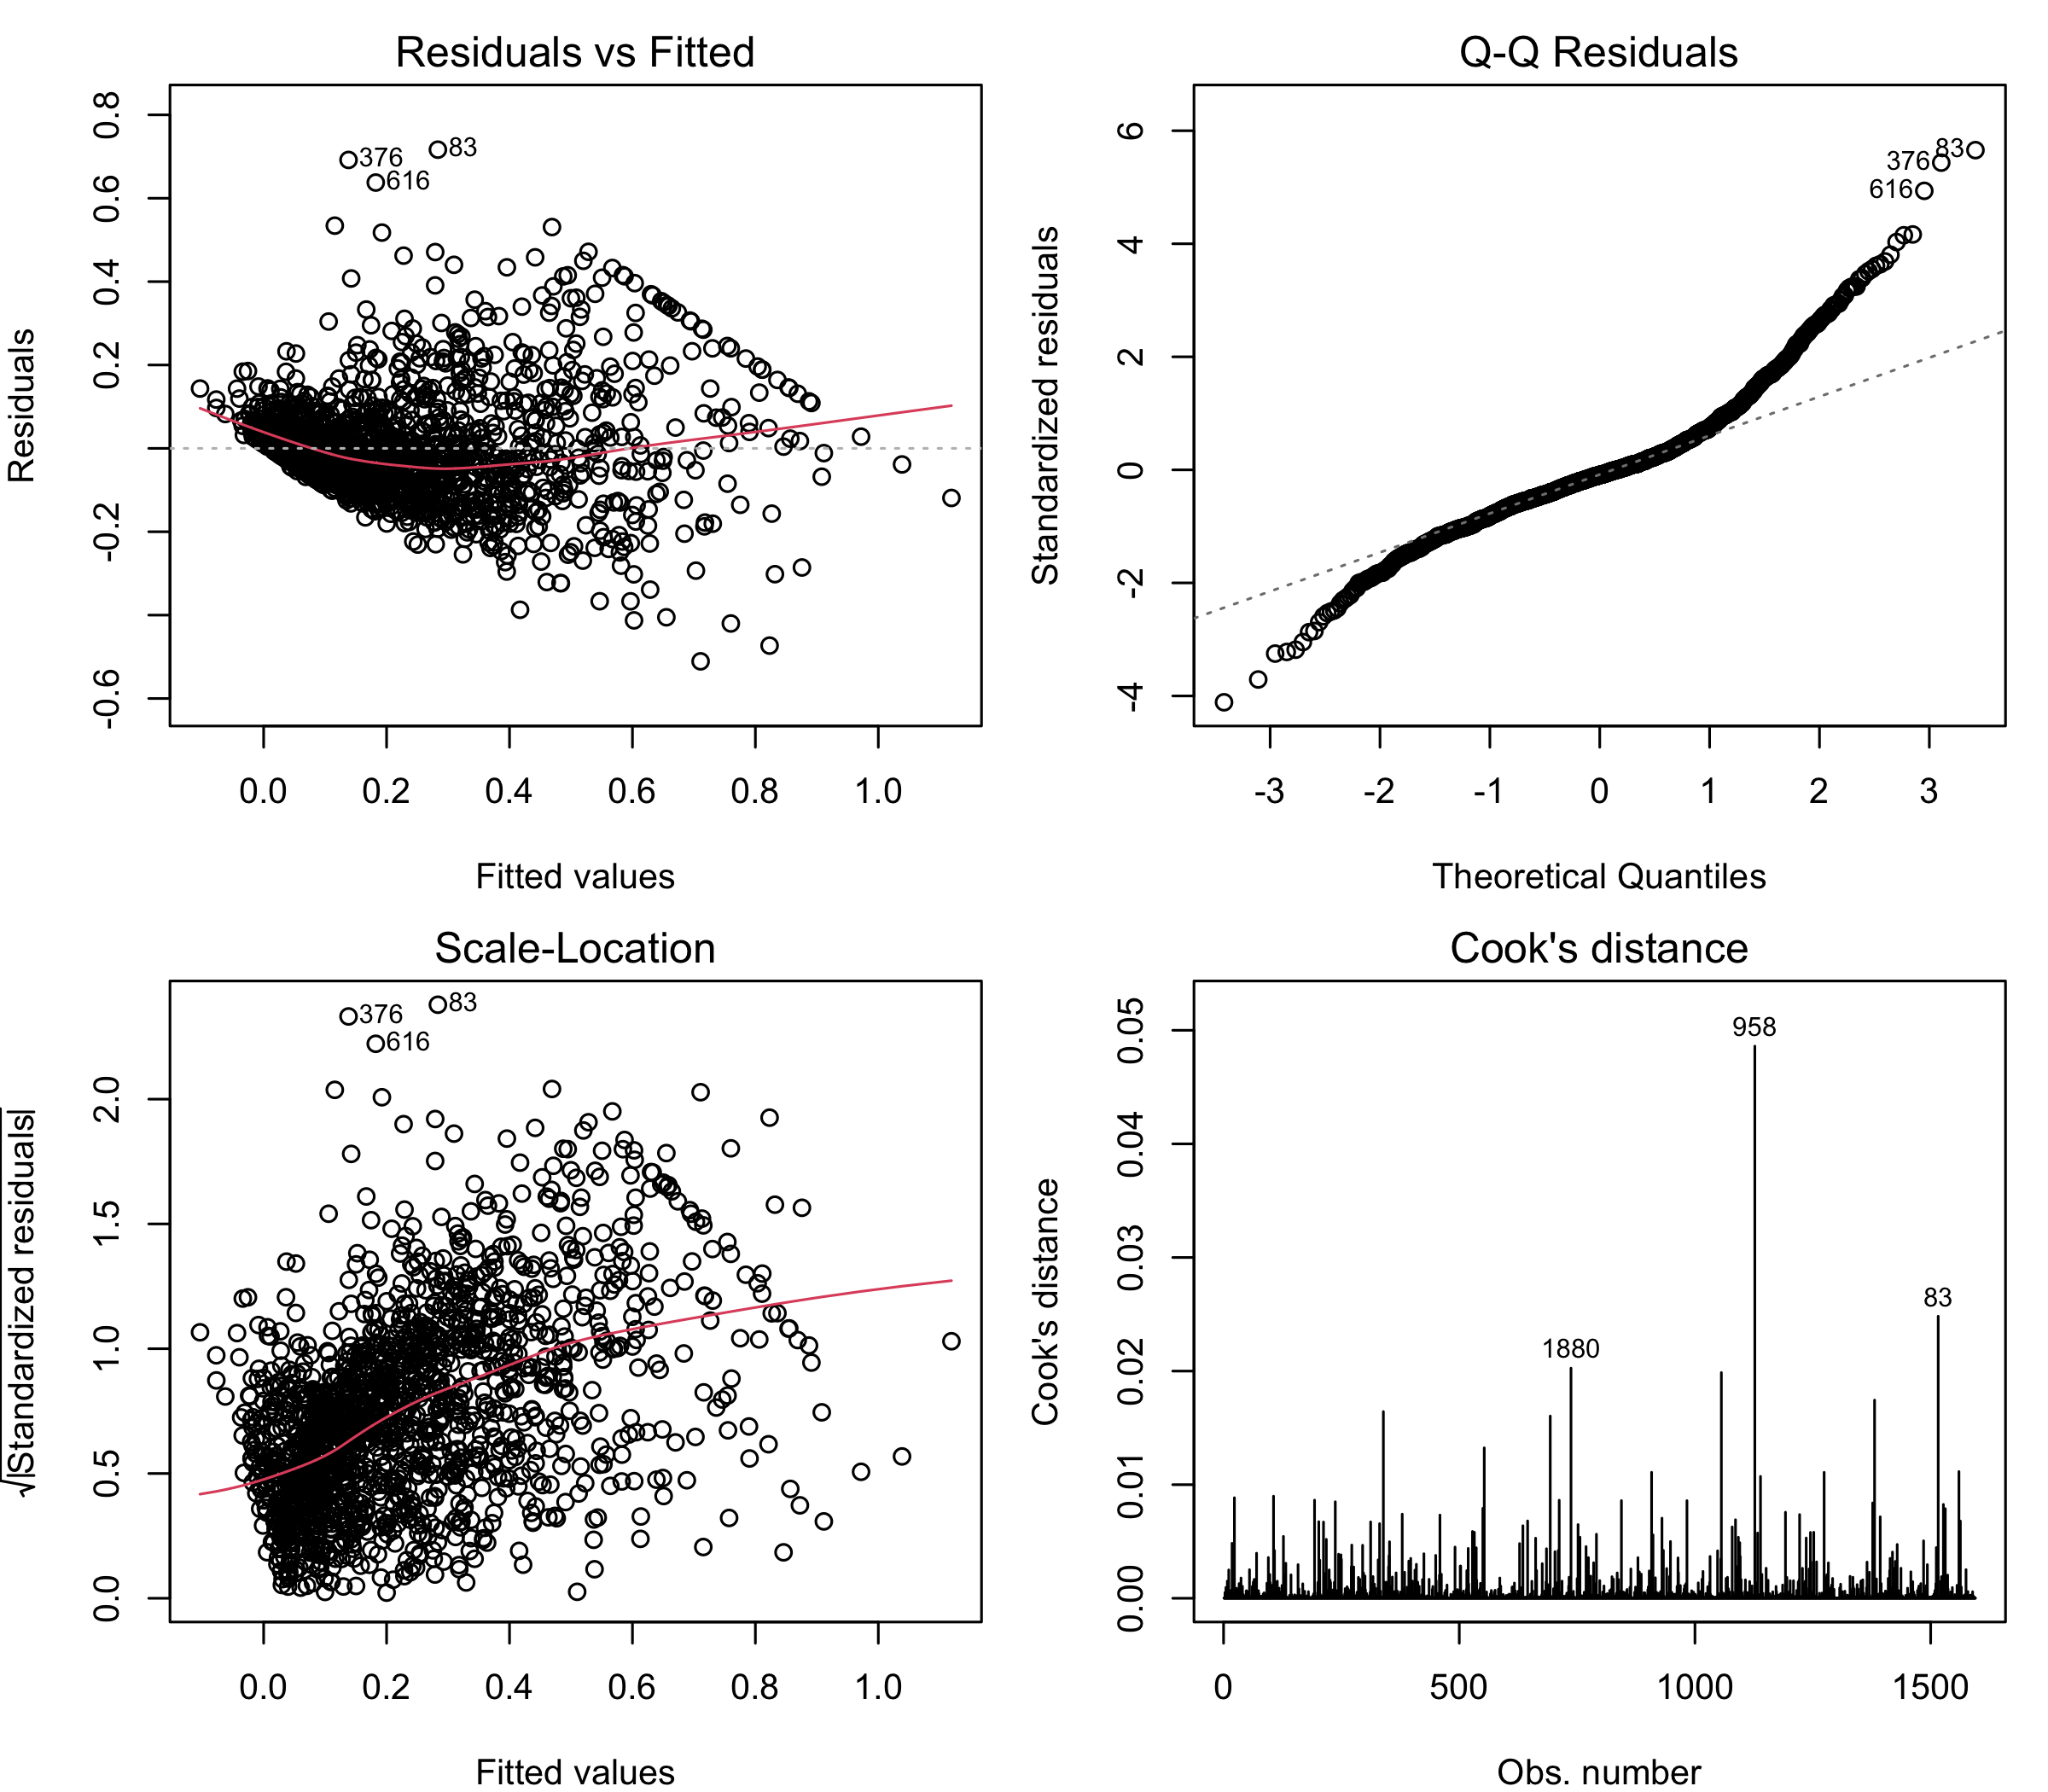
\includegraphics[width=\linewidth,keepaspectratio]{img/crime-ols-assumptions-1.png} \end{center}

\begin{longtable}[t]{ll}
\caption{\label{tab:ols-assumptions}Chẩn đoán mô hình OLS.}\\
\toprule
Kiểm định / chỉ tiêu & Kết quả\\
\midrule
Breusch–Pagan (phương sai đồng nhất) & BP = 307.5, p < 1e-16\\
Shapiro–Wilk (phần dư chuẩn) & W = 0.935, p < 1e-16\\
Số hệ số p < 0.05 với HC3 & 18\\
Cook's D lớn nhất & 0.049\\
Số quan sát $D_i > 4/n$ & 118\\
\addlinespace
Số quan sát $D_i > 0.5$ & 0\\
\bottomrule
\end{longtable}

\textbf{Nhận xét.}

\begin{itemize}
\tightlist
\item
  \textbf{Phương sai không đồng nhất}: Breusch--Pagan bác bỏ mạnh
  \(H_0\) (\(p < 10^{-16}\)); đồ thị Scale--Location cho thấy phương sai
  phần dư tăng theo giá trị dự đoán và điều này thường gặp khi biến phản
  hồi lệch phải và bị chặn dưới tại 0.
\item
  \textbf{Phần dư không chuẩn}: Shapiro--Wilk bác bỏ tính chuẩn
  (\(p < 10^{-16}\)), Q--Q plot lệch ở hai đuôi (một phần do 2.2\% quan
  sát bị dồn tại trần \(y = 1\)).
\item
  \textbf{Hệ quả}: không chuẩn chủ yếu ảnh hưởng suy diễn mẫu nhỏ;
  phương sai không đồng nhất làm sai số chuẩn cổ điển không đáng tin.
  Bản thân hai hiện tượng này không làm OLS chệch nếu
  \(E(\varepsilon\mid X)=0\), nhưng điều kiện đó không thể được chứng
  minh từ dữ liệu. Vì vậy báo cáo dùng HC3 cho suy diễn và validation
  cho đánh giá dự đoán.
\item
  \textbf{Quan sát ảnh hưởng}: khoảng cách Cook lớn nhất chỉ 0.049 và
  thấp hơn ngưỡng nghiêm trọng 0.5 hơn một bậc; 118 quan sát vượt ngưỡng
  thô \(4/n\) nhưng không quan sát nào chi phối kết quả ước lượng. Điều
  này \textbf{củng cố quyết định giữ toàn bộ quan sát} ở phần ngoại lai:
  các giá trị ``ngoại lai'' phân tán đều, không có điểm đòn bẩy đơn lẻ
  nào bóp méo mô hình.
\end{itemize}

\subsubsection{Ridge Regression}\label{ridge-regression}

Với \(\mathbf X_s\) và \(\mathbf y_c\) đã định nghĩa ở phần PCR, Ridge
giải đúng hàm mục tiêu mà \texttt{glmnet} sử dụng:

\[
\hat{\boldsymbol\beta}^{ridge}_\lambda
=\arg\min_{\boldsymbol\beta}\left\{
\frac{1}{2n}\|\mathbf y_c-\mathbf X_s\boldsymbol\beta\|_2^2
+\frac{\lambda}{2}\|\boldsymbol\beta\|_2^2\right\}
=(\mathbf X_s^\top\mathbf X_s+n\lambda\mathbf I)^{-1}\mathbf X_s^\top\mathbf y_c.
\]

Hệ số chặn \(\hat\beta_0=\bar y\) không bị phạt. Phần
\(n\lambda\mathbf I\) làm mọi trị riêng dương và co liên tục các hệ số
về 0.

\subsubsection{LASSO}\label{lasso}

LASSO thay phạt \(\ell_2\) bằng \(\ell_1\):

\[
\hat{\boldsymbol\beta}^{lasso}_\lambda
=\arg\min_{\boldsymbol\beta}\left\{
\frac{1}{2n}\|\mathbf y_c-\mathbf X_s\boldsymbol\beta\|_2^2
+\lambda\|\boldsymbol\beta\|_1\right\}.
\]

LASSO phạt tổng trị tuyệt đối của các hệ số. Cách phạt này có xu hướng
kéo một số hệ số nhỏ về đúng 0, nên các biến tương ứng bị loại khỏi mô
hình. Vì vậy LASSO vừa làm hệ số nhỏ lại, vừa thực hiện chọn biến tự
động.

\subsubsection{Chọn tham số phạt bằng kiểm chứng
chéo}\label{chux1ecdn-tham-sux1ed1-phux1ea1t-bux1eb1ng-kiux1ec3m-chux1ee9ng-chuxe9o}

\(\lambda\) của cả hai mô hình được chọn bằng kiểm chứng chéo 10-fold
trên tập huấn luyện, dùng \textbf{cùng một phân hoạch fold}
(\texttt{foldid}) để hai đường cong CV so sánh được với nhau. Ta báo cáo
cả \(\lambda_{\min}\) (cực tiểu sai số CV) và \(\lambda_{1se}\) (quy tắc
một sai số chuẩn).

\begin{center}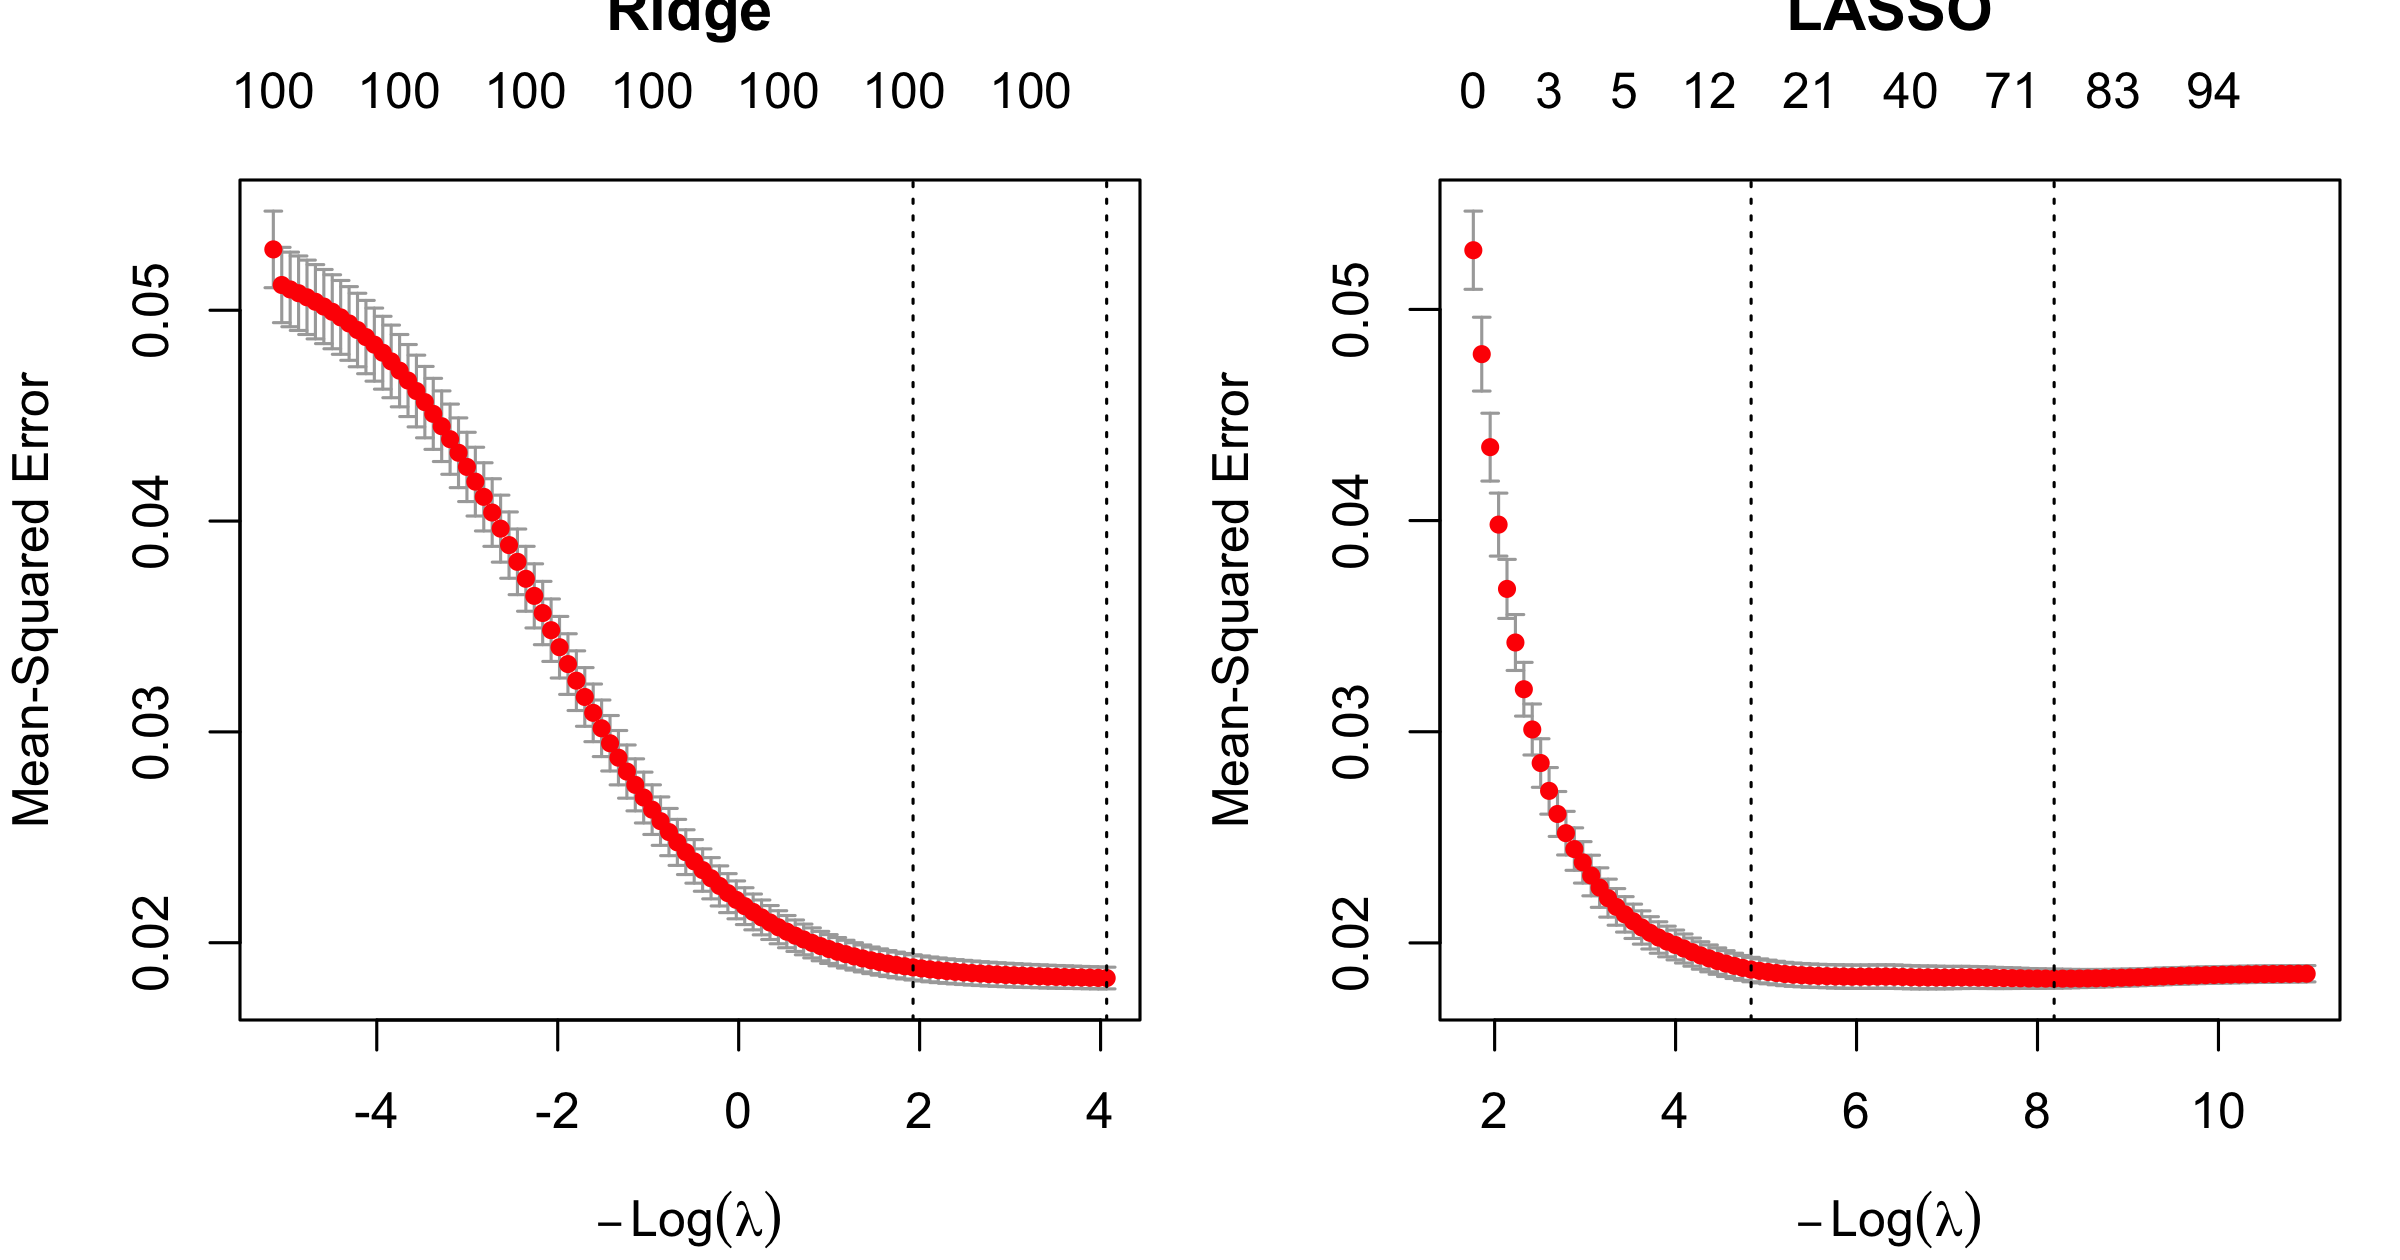
\includegraphics[width=\linewidth,keepaspectratio]{img/crime-glmnet-cv-1.png} \end{center}

\begin{longtable}[t]{llrrr}
\caption{\label{tab:glmnet-cv}Tham số phạt chọn bằng kiểm chứng chéo 10-fold (cùng foldid).}\\
\toprule
Mô hình & Quy tắc & $\lambda$ & MSE (CV) & Số hệ số khác 0\\
\midrule
Ridge & $\lambda_{\min}$ & 0.0171 & 0.0183 & 100\\
Ridge & $\lambda_{1se}$ & 0.1460 & 0.0188 & 100\\
LASSO & $\lambda_{\min}$ & 0.0003 & 0.0183 & 76\\
LASSO & $\lambda_{1se}$ & 0.0080 & 0.0187 & 14\\
\bottomrule
\end{longtable}

\textbf{Nhận xét.} Với Ridge, \(\lambda_{\min} = 0.0171\) khá nhỏ, bên
cạnh đó dữ liệu với \(n = 1595 \gg p = 100\) không đòi hỏi co hệ số quá
mạnh. Với LASSO, \(\lambda_{\min} = \ensuremath{2.79\times 10^{-4}}\)
giữ 76 biến, còn \(\lambda_{1se} = 0.00795\) chỉ giữ \textbf{14 biến} ,
một mô hình cực gọn sẽ rất hữu ích khi diễn giải. Để so sánh khả năng dự
đoán thuần túy ở mục sau, ta dùng \(\lambda_{\min}\) cho cả hai mô hình
(đây là giá trị tối ưu hóa sai số CV); các phương án \(\lambda_{1se}\)
được báo cáo kèm để tham khảo.

\subsection{Đánh giá và so sánh mô hình trên tập kiểm
định}\label{ux111uxe1nh-giuxe1-vuxe0-so-suxe1nh-muxf4-huxecnh-truxean-tux1eadp-kiux1ec3m-ux111ux1ecbnh}

Ba chỉ số đánh giá trên tập kiểm định (\(n_{val} = 399\)), với
\(\hat y_i\) là giá trị dự đoán:

\[
\mathrm{RMSE} = \sqrt{\tfrac{1}{n}\textstyle\sum_i (y_i - \hat y_i)^2}, \qquad
\mathrm{MAE} = \tfrac{1}{n}\textstyle\sum_i |y_i - \hat y_i|, \qquad
R^2 = 1 - \frac{\sum_i (y_i - \hat y_i)^2}{\sum_i (y_i - \bar y_{val})^2}.
\]

RMSE phạt nặng sai số lớn, MAE bền vững hơn với sai số cực đoan; \(R^2\)
ở đây là tỷ lệ phương sai của \(y\) trên tập kiểm định được mô hình giải
thích (quy ước \(\bar y_{val}\) ở mẫu số).

\begin{table}[H]
\centering
\caption{So sánh hiệu năng của bốn mô hình trên tập kiểm định}
\label{tab:danh-gia}
\begin{tabular}{lccc}
\toprule
\textbf{Mô hình}
  & \textbf{RMSE} $\downarrow$
  & \textbf{MAE} $\downarrow$
  & $\boldsymbol{R^2}$ $\uparrow$ \\
\midrule
PCR ($k=12$)                & 0.1479          & 0.1065          & 0.6314 \\
OLS                         & 0.1386          & \textbf{0.0990} & 0.6765 \\
Ridge ($\lambda_{\min}$)   & 0.1396          & 0.1005          & 0.6714 \\
\textbf{LASSO ($\lambda_{\min}$)}
                            & \textbf{0.1379} & \textbf{0.0990} & \textbf{0.6794} \\
\bottomrule
\end{tabular}
\end{table}

\begin{longtable}[t]{lrrr}
\caption{\label{tab:danh-gia-1se}Tham khảo: các phương án $\lambda_{1se}$ gọn hơn.}\\
\toprule
Mô hình & RMSE & MAE & R2\\
\midrule
Ridge ($\lambda_{1se}$) & 0.1443 & 0.1038 & 0.6489\\
LASSO ($\lambda_{1se}$) & 0.1447 & 0.1021 & 0.6472\\
\bottomrule
\end{longtable}

\begin{longtable}[t]{lrlrl}
\caption{\label{tab:bootstrap-delta}Chênh lệch sai số so với LASSO và khoảng tin cậy bootstrap ghép cặp.}\\
\toprule
So sánh với LASSO & $\Delta$RMSE & KTC 95\% $\Delta$RMSE & $\Delta$MAE & KTC 95\% $\Delta$MAE\\
\midrule
PCR & 0.0100 & {}[0.0054; 0.0142] & 0.0074 & {}[0.0035; 0.0115]\\
OLS & 0.0006 & {}[-0.0011; 0.0023] & 0.0000 & {}[-0.0017; 0.0017]\\
Ridge & 0.0017 & {}[0.0001; 0.0034] & 0.0015 & {}[-0.0002; 0.0031]\\
\bottomrule
\end{longtable}

\begin{center}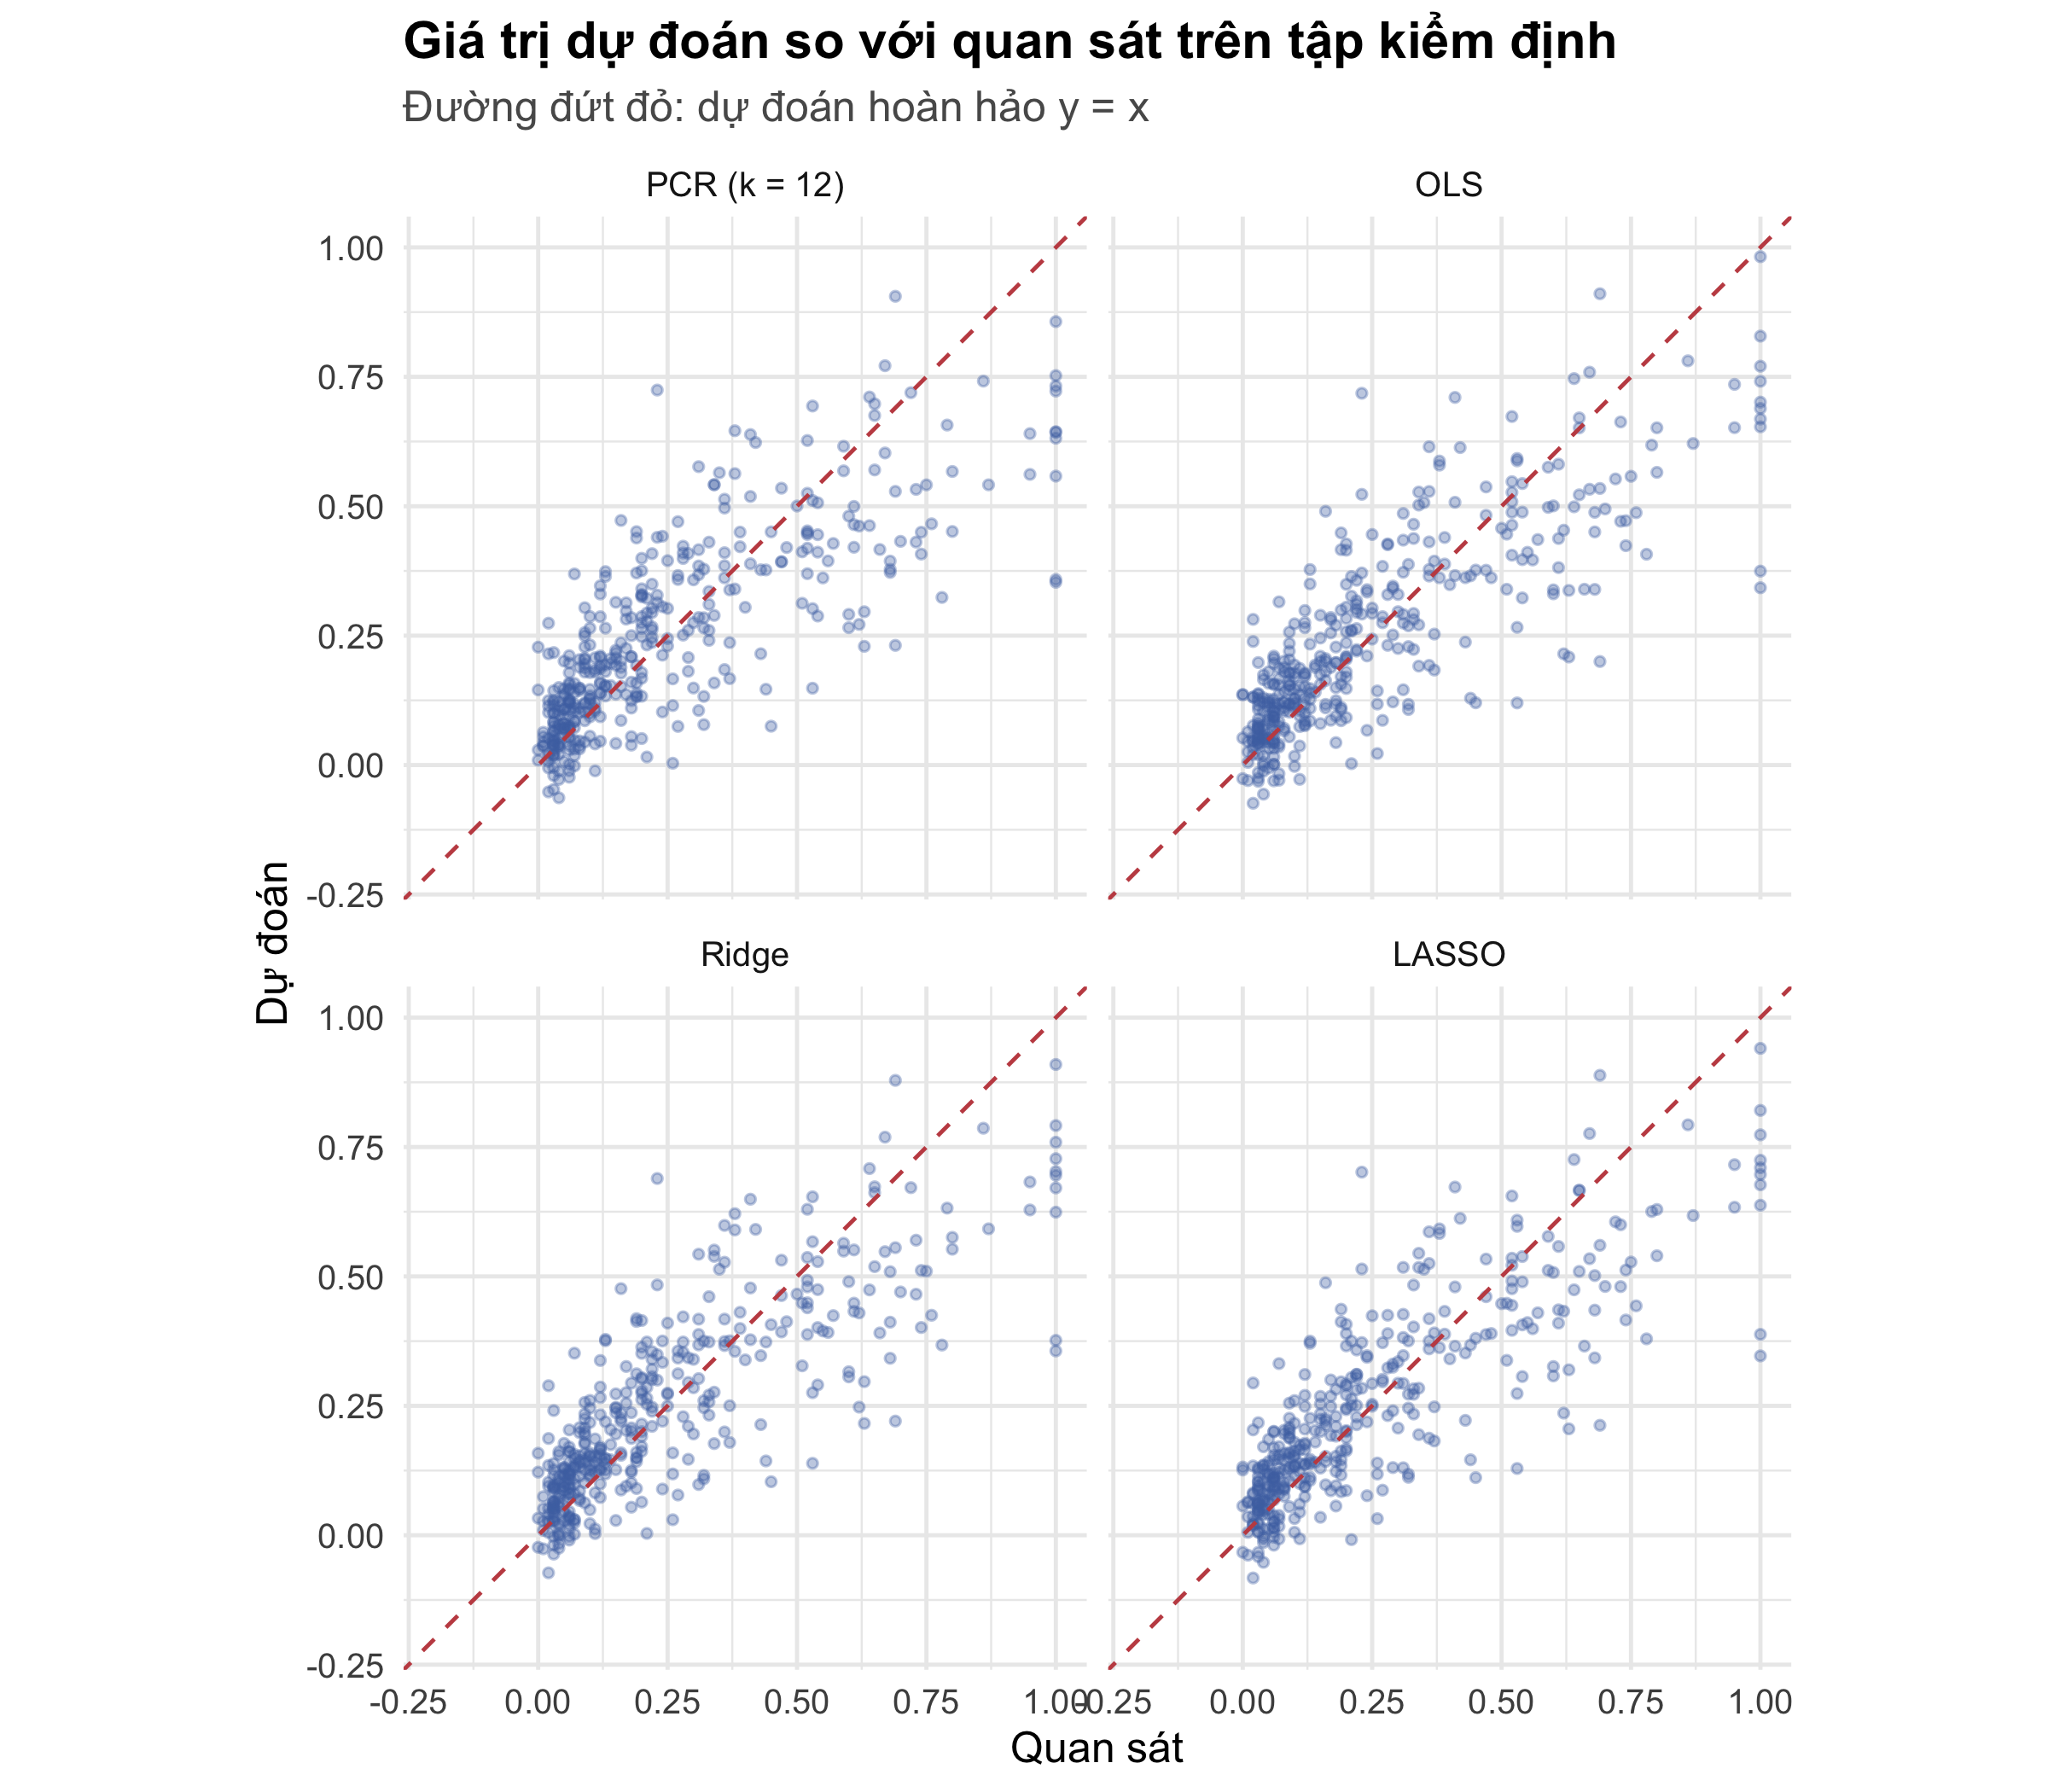
\includegraphics[width=\linewidth,keepaspectratio]{img/crime-pred-vs-obs-1.png} \end{center}

\textbf{Nhận xét.}

\begin{itemize}
\tightlist
\item
  \textbf{LASSO (\(\lambda_{\min}\)) có sai số điểm thấp nhất} (RMSE
  \(= 0.1379\), \(R^2 = 0.6794\)), nhưng khoảng cách với OLS và Ridge
  nhỏ. Bảng bootstrap cho biết độ bất định của các chênh lệch này trên
  tập validation; khoảng chứa 0 không cung cấp bằng chứng rõ về ưu thế
  của một mô hình.
\item
  \textbf{PCR (\(k = 12\)) có sai số lớn nhất} (RMSE \(= 0.1479\),
  \(R^2 = 0.6314\)): các thành phần có phương sai lớn của \(\mathbf X\)
  không nhất thiết chứa toàn bộ tín hiệu dự đoán cho \(y\).
\item
  Trên đồ thị dự đoán--quan sát, cả bốn mô hình co dự đoán về trung tâm
  và có thể dự đoán ngoài \([0,1]\), vì mô hình tuyến tính không áp ràng
  buộc miền giá trị.
\item
  MAE (0.099 với LASSO) nhỏ hơn RMSE ở mọi mô hình, cho thấy một nhóm
  sai số lớn kéo RMSE lên.
\end{itemize}

Khoảng bootstrap ở đây là \textbf{có điều kiện trên các mô hình đã
khớp}; nó chưa phản ánh biến thiên do chia lại train/validation hoặc
huấn luyện lại mô hình.

\subsection{Phân tích các thành phần chính qua ma trận
tải}\label{phuxe2n-tuxedch-cuxe1c-thuxe0nh-phux1ea7n-chuxednh-qua-ma-trux1eadn-tux1ea3i}

Vector tải \(\mathbf{v}_j\) cho biết mỗi thành phần chính là tổ hợp
tuyến tính nào của các biến gốc (đã chuẩn hóa); vì
\(\lVert\mathbf{v}_j\rVert = 1\), độ lớn \(|v_{ij}|\) đo mức đóng góp
tương đối của biến \(i\) vào thành phần \(j\). Ta xét 4 thành phần đầu
(chiếm 58.7\% phương sai) qua 10 biến có \(|v_{ij}|\) lớn nhất của mỗi
thành phần, đồng thời tính \textbf{tương quan giữa điểm thành phần
(scores) với \(y\)} để đo mức liên quan của từng thành phần tới tội
phạm.

\begin{longtable}[t]{lrlr}
\caption{\label{tab:loadings-tables}10 biến tải lớn nhất của PC1 (PVE 25.2\%) và PC2 (PVE 16.5\%).}\\
\toprule
Biến (PC1) & v1 & Biến (PC2) & v2\\
\midrule
medFamInc & -0.184 & PctRecImmig8 & -0.221\\
medIncome & -0.183 & PctRecImmig10 & -0.221\\
PctKids2Par & -0.174 & PctRecImmig5 & -0.219\\
pctWInvInc & -0.174 & PctRecentImmig & -0.216\\
PctPopUnderPov & 0.173 & PctForeignBorn & -0.213\\
\addlinespace
PctYoungKids2Par & -0.171 & PctSpeakEnglOnly & 0.192\\
PctFam2Par & -0.171 & PctNotSpeakEnglWell & -0.187\\
perCapInc & -0.170 & PctPersDenseHous & -0.175\\
PctHousNoPhone & 0.165 & racePctAsian & -0.166\\
pctWPubAsst & 0.164 & racePctHisp & -0.161\\
\bottomrule
\end{longtable}

\begin{longtable}[t]{lrlr}
\caption{\label{tab:loadings-tables-pc34}10 biến tải lớn nhất của PC3 (PVE 9.4\%) và PC4 (PVE 7.5\%).}\\
\toprule
Biến (PC3) & v3 & Biến (PC4) & v4\\
\midrule
PersPerOccupHous & 0.259 & PctSameCity85 & 0.259\\
PersPerFam & 0.237 & agePct12t29 & -0.251\\
householdsize & 0.226 & PctSameHouse85 & 0.247\\
PersPerOwnOccHous & 0.225 & agePct16t24 & -0.242\\
PersPerRentOccHous & 0.211 & agePct12t21 & -0.238\\
\addlinespace
PctLargHouseOccup & 0.210 & agePct65up & 0.195\\
PctLargHouseFam & 0.178 & pctWSocSec & 0.186\\
HousVacant & -0.166 & PctSameState85 & 0.178\\
numbUrban & -0.149 & PctImmigRec5 & -0.177\\
population & -0.148 & PctImmigRecent & -0.177\\
\bottomrule
\end{longtable}

\begin{center}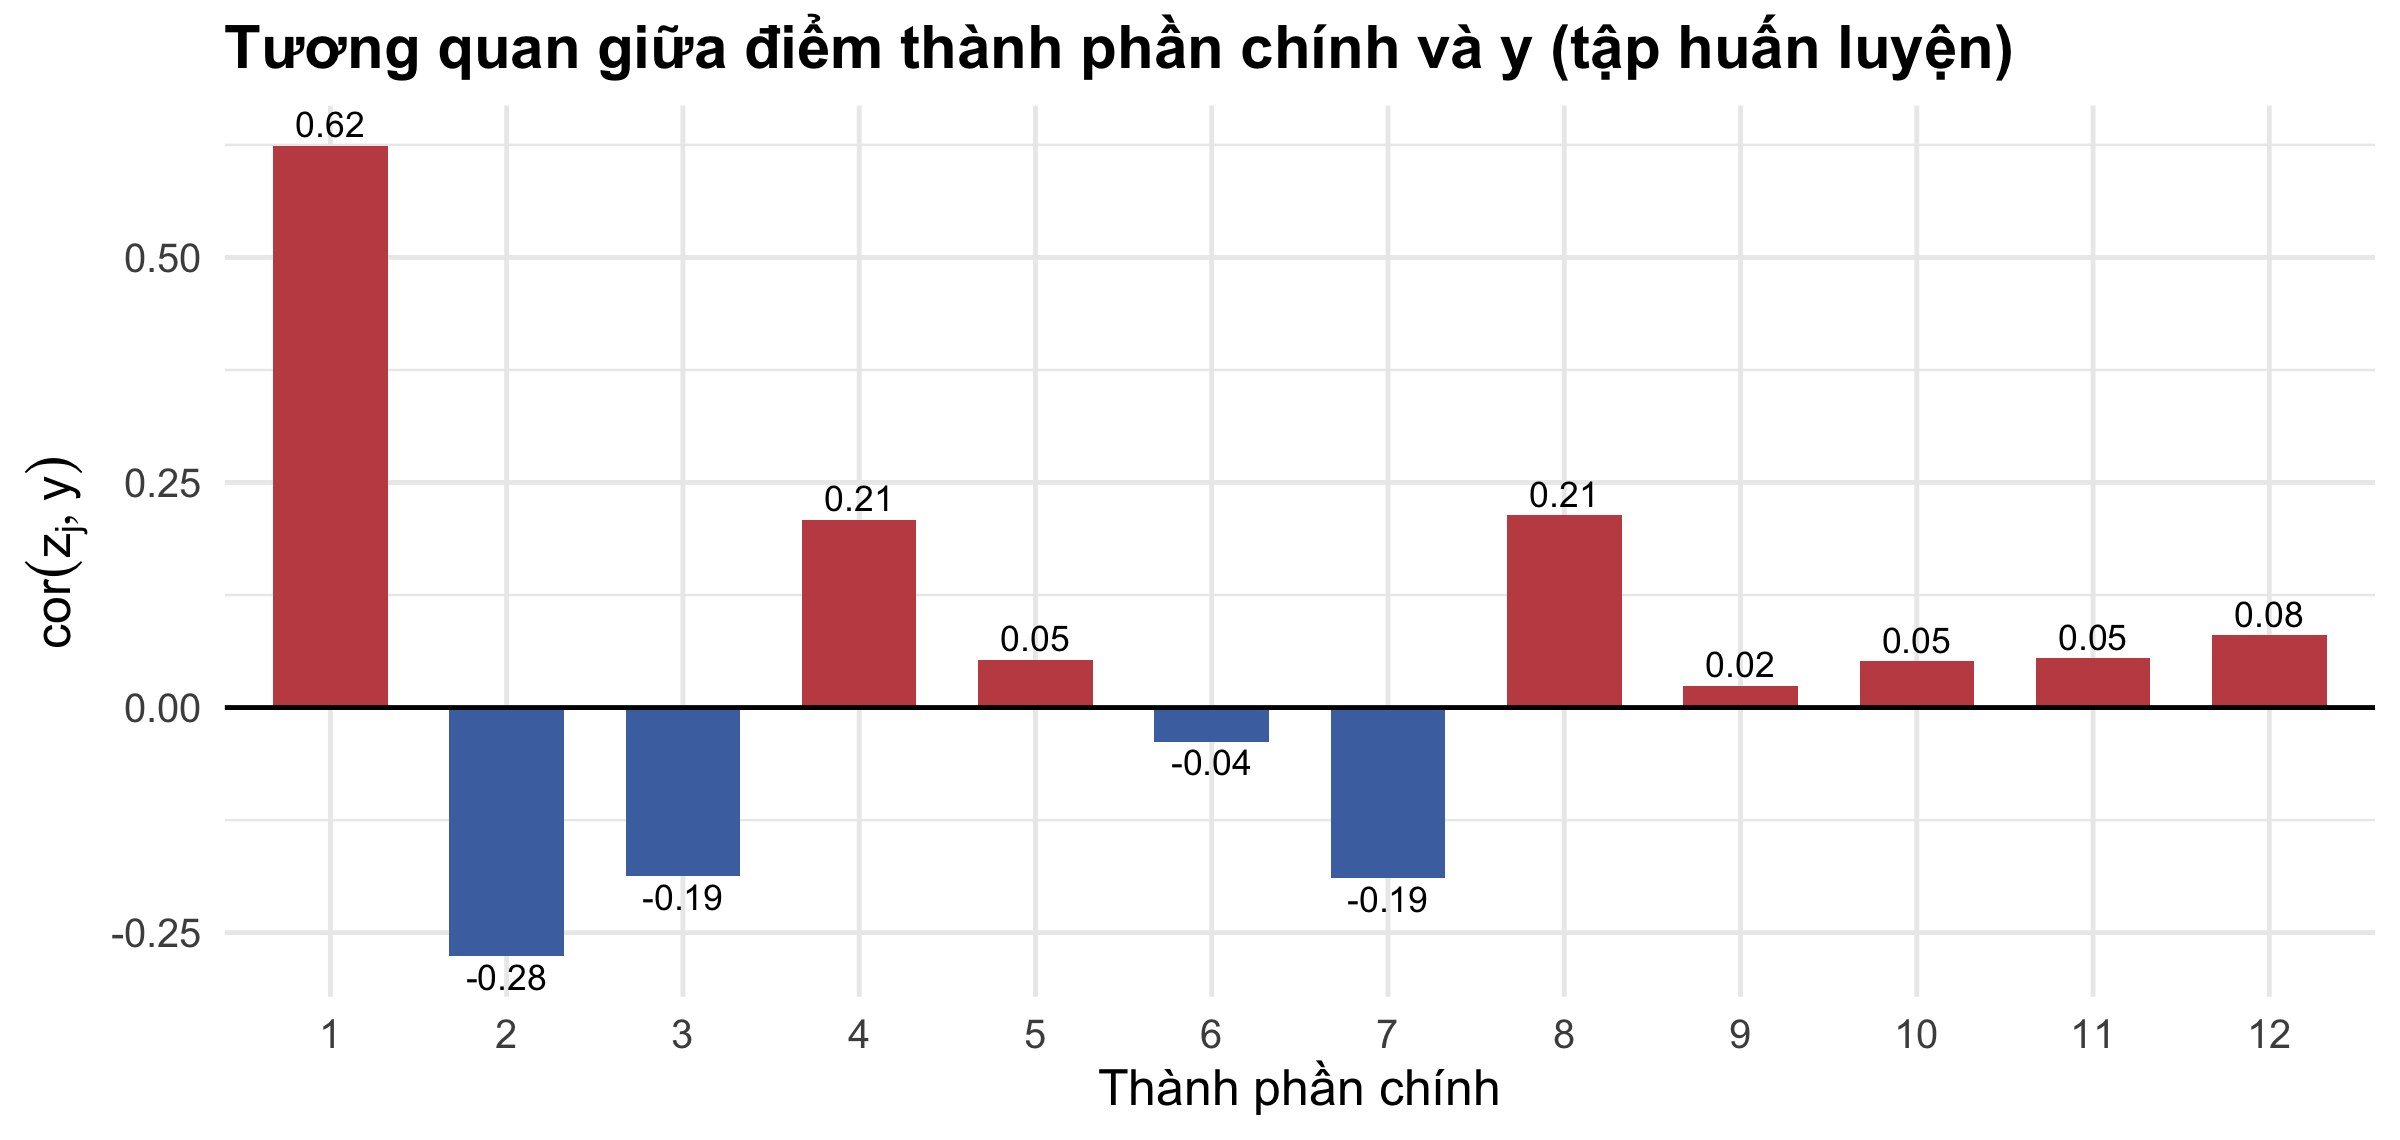
\includegraphics[width=\linewidth,keepaspectratio]{img/crime-pc-cor-y-1.png} \end{center}

\textbf{Diễn giải các thành phần} (dựa trên các bảng tải ở trên, đối
chiếu với bảng nhóm biến):

\begin{itemize}
\tightlist
\item
  \textbf{PC1 --- trục ``bất lợi kinh tế và cấu trúc gia đình''} (PVE
  25.2\%): tải \textbf{âm} với mọi biến thu nhập (\texttt{medFamInc},
  \texttt{medIncome}, \texttt{pctWInvInc}, \texttt{perCapInc}) và biến
  gia đình đủ hai bố mẹ (\texttt{PctKids2Par}, \texttt{PctFam2Par}); tải
  \textbf{dương} với nghèo đói và trợ cấp (\texttt{PctPopUnderPov},
  \texttt{pctWPubAsst}, \texttt{PctHousNoPhone}). Giá trị PC1 cao tương
  đương cộng đồng nghèo, ít gia đình nguyên vẹn. Đây cũng là thành phần
  liên hệ mạnh nhất với tội phạm: \(\mathrm{cor}(z_1, y) = 0.62\) , có
  thể nói đây là \textbf{một trục tóm tắt phần lớn tín hiệu chính} mà
  EDA đã thấy ở phần tương quan.
\item
  \textbf{PC2 --- trục ``nhập cư và ngôn ngữ''} (PVE 16.5\%): tải âm
  đồng loạt với các biến nhập cư gần đây (\texttt{PctRecImmig5/8/10},
  \texttt{PctForeignBorn}, \texttt{PctNotSpeakEnglWell}) và dương với
  \texttt{PctSpeakEnglOnly}; giá trị cao tương đương cộng đồng ``bản
  địa'', ít dân nhập cư. Tương quan với \(y\) ở mức vừa (\(-0.28\)).
\item
  \textbf{PC3 --- trục ``quy mô hộ và nhà ở đông người''} (PVE 9.4\%):
  các biến người/hộ (\texttt{PersPerOccupHous}, \texttt{PersPerFam},
  \texttt{householdsize}, \texttt{PctLargHouseOccup}) tải dương mạnh.
\item
  \textbf{PC4 --- trục ``ổn định cư trú và cơ cấu tuổi''} (PVE 7.5\%):
  dương với các biến ở lâu một chỗ (\texttt{PctSameCity85},
  \texttt{PctSameHouse85}) và dân số già (\texttt{agePct65up},
  \texttt{pctWSocSec}), âm với các nhóm tuổi trẻ (\texttt{agePct12t29},
  \texttt{agePct16t24}).
\end{itemize}

\textbf{Nhận xét quan trọng cho PCR.} Biểu đồ tương quan thành
phần--\(y\) bộc lộ đúng yếu điểm của PCR: mức liên quan tới \(y\)
\textbf{không giảm dần theo thứ tự phương sai}. Chẳng hạn PC8 chỉ chiếm
2.9\% phương sai nhưng có \(\mathrm{cor}(z_8, y) = 0.21\), vốn ngang với
PC4 và cao hơn hẳn PC5, PC6 (gần như bằng 0). PCA sắp xếp các thành phần
theo lượng phương sai của \(\mathbf{X}\), không theo giá trị dự đoán cho
\(y\); vì vậy quy tắc ``giữ \(k\) thành phần đầu'' có thể vừa giữ những
thành phần ít liên quan tới \(y\)

\subsection{Chuyển hệ số PCR về không gian biến
gốc}\label{chuyux1ec3n-hux1ec7-sux1ed1-pcr-vux1ec1-khuxf4ng-gian-biux1ebfn-gux1ed1c}

\subsubsection{Công thức chuyển
đổi}\label{cuxf4ng-thux1ee9c-chuyux1ec3n-ux111ux1ed5i}

Mô hình PCR trên không gian thành phần là
\(\hat y = \bar y + \mathbf{z}^\top\hat{\boldsymbol\gamma}\) với
\(\mathbf{z} = \mathbf{V}_k^\top \mathbf{x}_s\). Thay ngược, hệ số trên
\textbf{biến chuẩn hóa} là
\(\hat{\boldsymbol\beta}^{std} = \mathbf{V}_k\hat{\boldsymbol\gamma}\),
và quy về \textbf{thang đo gốc} của biến \(j\) (chia cho độ lệch chuẩn
huấn luyện \(s_j\), điều chỉnh hệ số chặn):

\[
\hat\beta_j = \frac{(\mathbf{V}_k\hat{\boldsymbol\gamma})_j}{s_j},
\qquad
\hat\beta_0 = \bar y_{train} - \sum_{j=1}^{p} \hat\beta_j\,\bar x_{j,train}.
\]

Do các cột điểm thành phần trực giao,
\(\hat\gamma_j = \mathbf{z}_j^\top\mathbf{y} / \mathbf{z}_j^\top\mathbf{z}_j\)
tính được từng thành phần độc lập. Ta thực hiện phép chuyển đổi thủ công
rồi \textbf{kiểm chứng bằng số}: dự đoán từ
\((\hat\beta_0, \hat{\boldsymbol\beta})\) phải trùng dự đoán của mô hình
\texttt{pls} đến sai số dấu phẩy động.

Sai số lớn nhất giữa hai cách tính là \(2.52e-14\) với cỡ sai số làm
tròn của số thực dấu phẩy động, xác nhận phép chuyển đổi chính xác.

\subsubsection{Diễn giải hệ số trên các biến
gốc}\label{diux1ec5n-giux1ea3i-hux1ec7-sux1ed1-truxean-cuxe1c-biux1ebfn-gux1ed1c}

Để so sánh hệ số \textbf{giữa các biến}, ta dùng \(\hat\beta^{std}\).
Trong mặt phẳng hồi quy đã khớp, tăng \(X_j\) một độ lệch chuẩn trong
khi giữ các biến khác cố định làm dự đoán thay đổi
\(\hat\beta^{std}_j\). Đây là liên hệ có điều kiện của mô hình, không
phải tác động nhân quả.

\begin{longtable}[t]{lrr}
\caption{\label{tab:beta-table}15 biến có hệ số PCR (chuẩn hóa) lớn nhất về trị tuyệt đối.}\\
\toprule
Biến & $\hat\beta^{std}$ & $\hat\beta$ (thang gốc)\\
\midrule
racepctblack & 0.0219 & 0.0860\\
racePctWhite & -0.0198 & -0.0822\\
PctIlleg & 0.0170 & 0.0745\\
PctKids2Par & -0.0148 & -0.0716\\
PctTeen2Par & -0.0146 & -0.0765\\
\addlinespace
PctFam2Par & -0.0137 & -0.0679\\
PctYoungKids2Par & -0.0127 & -0.0586\\
FemalePctDiv & 0.0122 & 0.0694\\
TotalPctDiv & 0.0117 & 0.0633\\
PctVacantBoarded & 0.0109 & 0.0517\\
\addlinespace
MalePctDivorce & 0.0102 & 0.0558\\
pctWPubAsst & 0.0085 & 0.0383\\
pctUrban & 0.0076 & 0.0170\\
PctEmplManu & -0.0070 & -0.0344\\
PctLargHouseFam & 0.0070 & 0.0363\\
\bottomrule
\end{longtable}

\begin{center}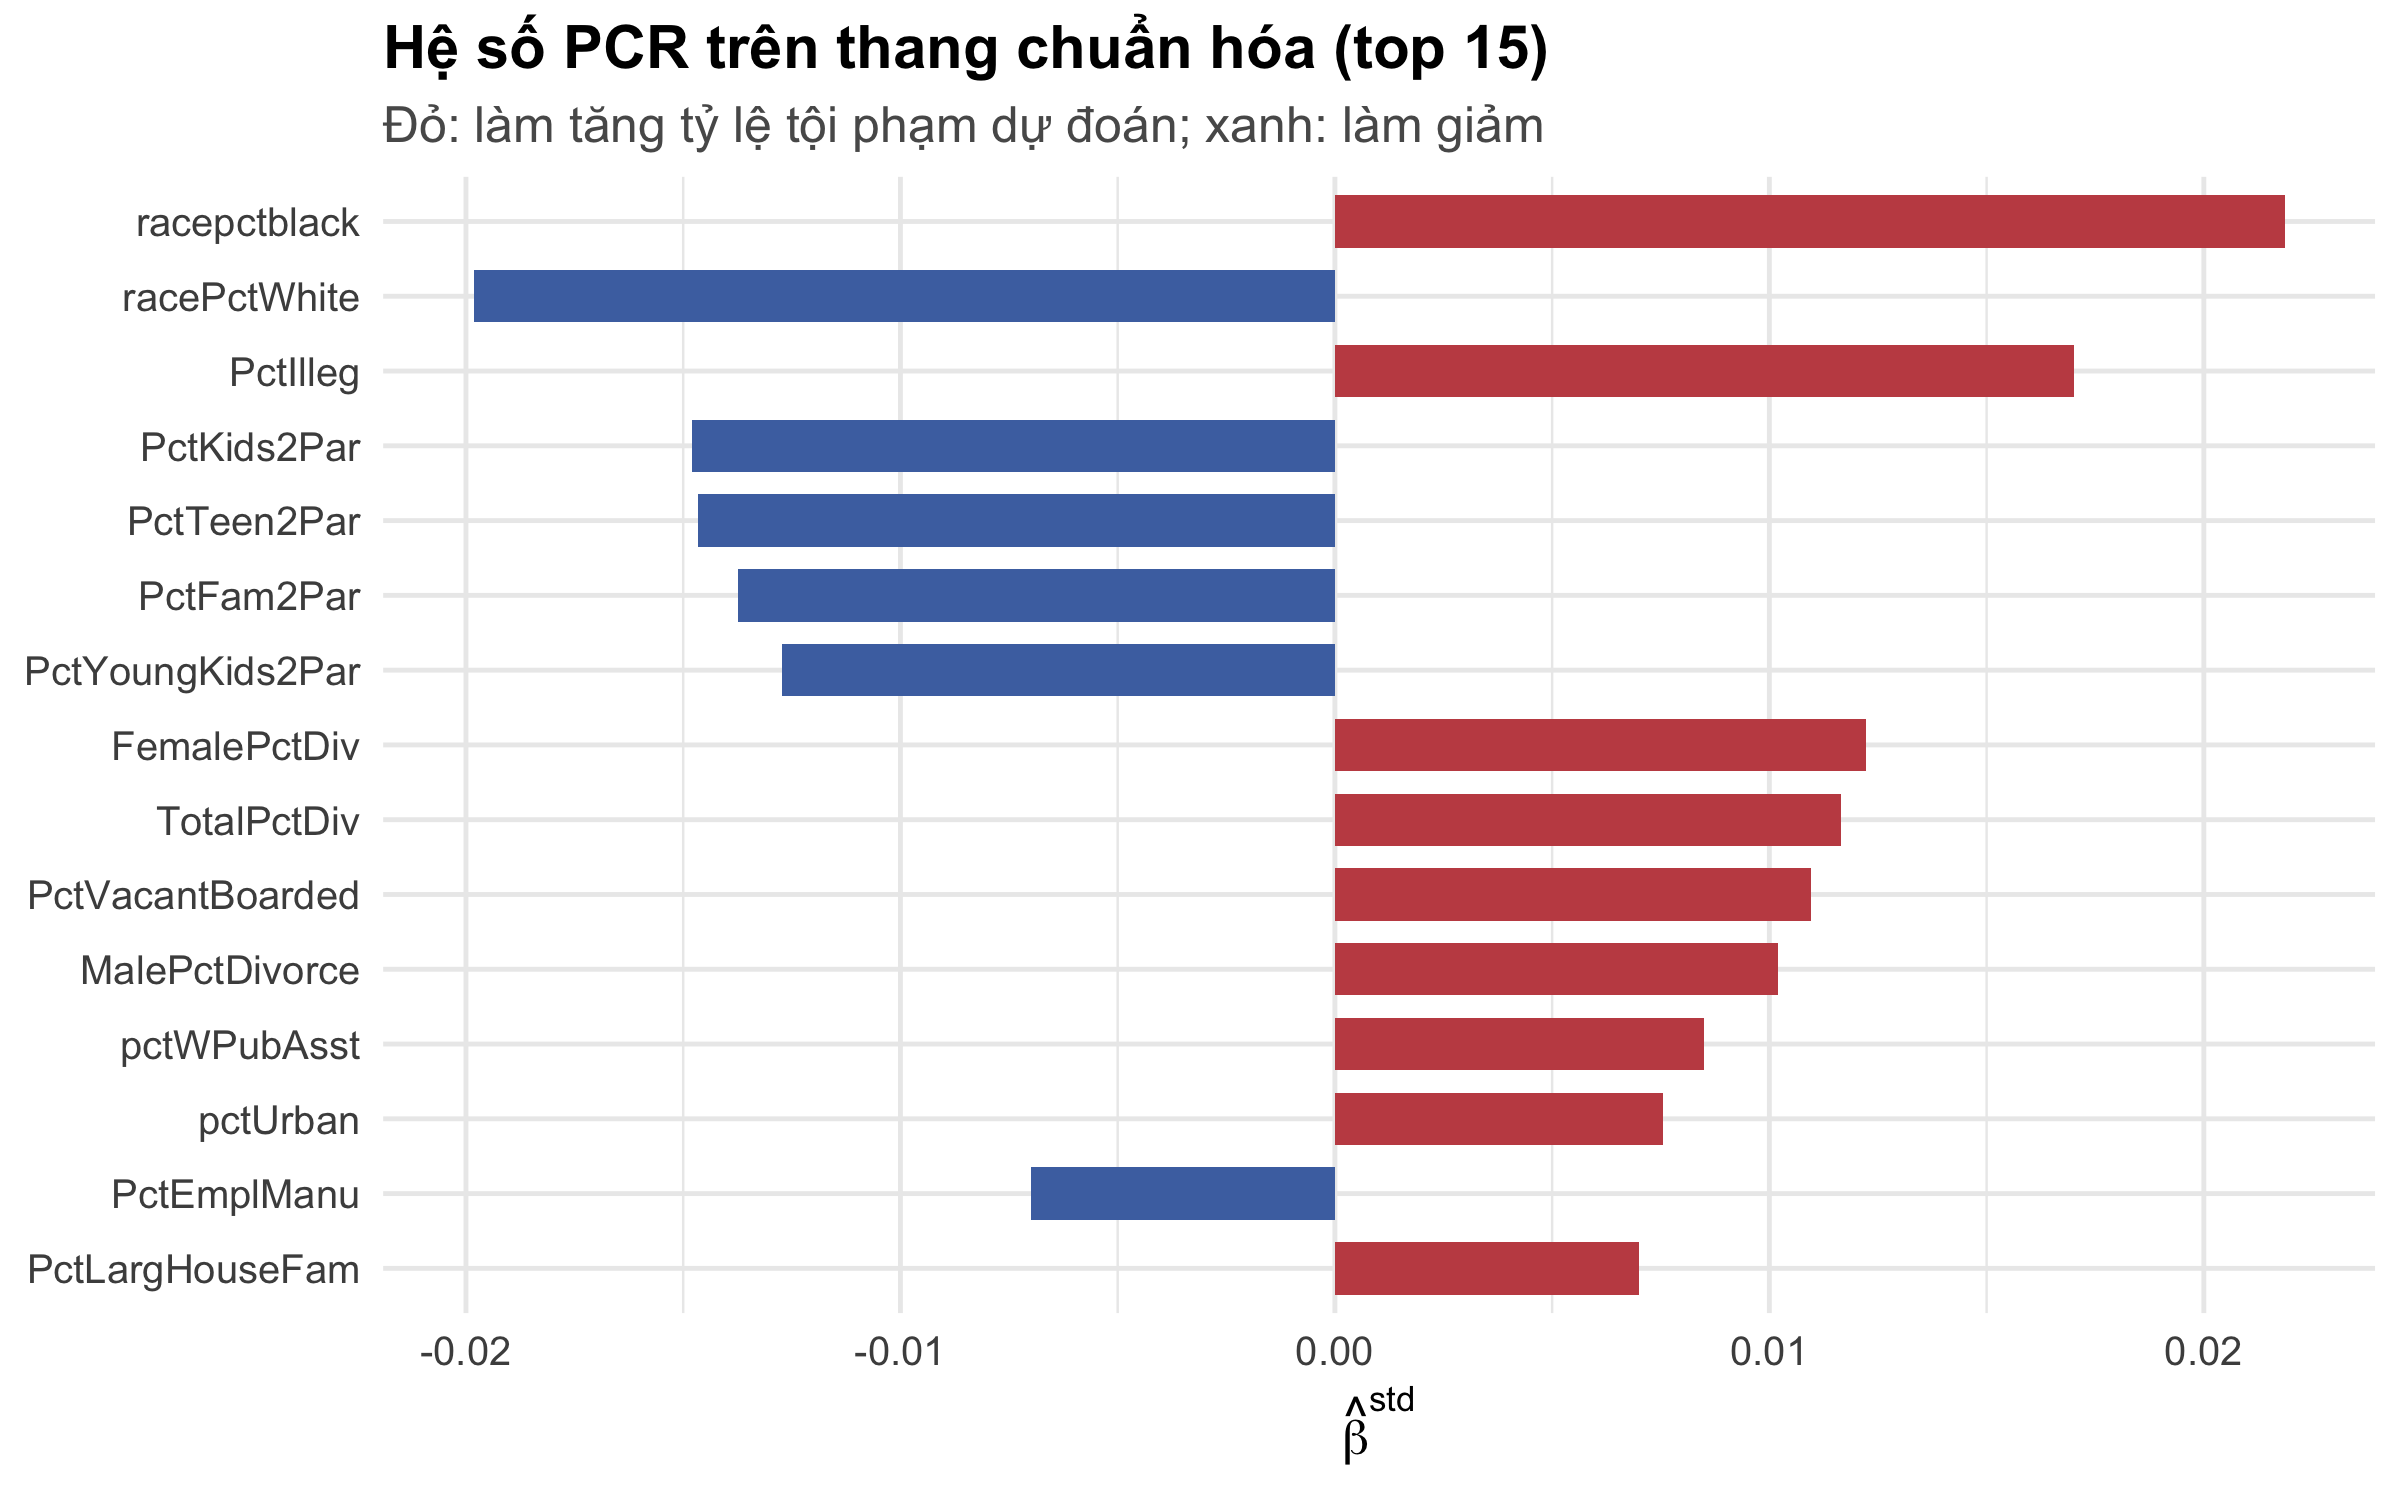
\includegraphics[width=\linewidth,keepaspectratio]{img/crime-beta-plot-1.png} \end{center}

\textbf{Diễn giải.} Các hệ số lớn nhất tập trung vào vài cụm nội dung,
nhìn chung nhất quán với phân tích tương quan ở phần EDA:

\begin{itemize}
\tightlist
\item
  \textbf{Cấu trúc gia đình} là cụm mạnh nhất: \texttt{PctIlleg} (con
  ngoài giá thú, \(+\)), bốn biến gia đình đủ hai bố mẹ
  \texttt{PctKids2Par}, \texttt{PctTeen2Par}, \texttt{PctFam2Par},
  \texttt{PctYoungKids2Par} (đều \(-\)), và cụm ly hôn
  \texttt{FemalePctDiv}, \texttt{TotalPctDiv}, \texttt{MalePctDivorce}
  (đều \(+\)). Đáng chú ý, PCR phân bổ trọng số khá đều cho cả bốn biến
  ``hai bố mẹ'' vốn tương quan rất cao, hệ quả tự nhiên của việc ước
  lượng qua các thành phần chung thay vì từng biến riêng.
\item
  \textbf{Cơ cấu chủng tộc}: \texttt{racepctblack} (\(+\)) và
  \texttt{racePctWhite} (\(-\)) đứng đầu bảng. Đây là liên hệ thống kê
  trong dữ liệu quan sát, không phải quan hệ nhân quả; trong dữ liệu Hoa
  Kỳ 1990, biến chủng tộc gắn chặt với các bất lợi cấu trúc như nghèo
  đói, nhà ở và cơ hội việc làm, nên mô hình không tách được các hiệu
  ứng này.
\item
  \textbf{Suy thoái nhà ở và bất lợi đô thị}: \texttt{PctVacantBoarded}
  (nhà bỏ hoang bịt ván, \(+\)), cùng với \texttt{pctWPubAsst} (\(+\))
  và \texttt{pctUrban} (\(+\)), cho thấy các dấu hiệu bất lợi kinh tế -
  đô thị vẫn nằm trong nhóm hệ số lớn. Diễn giải này là liên hệ thống kê
  trong dữ liệu quan sát, không nên hiểu như tác động nhân quả.
\end{itemize}

\subsubsection{Đối chiếu với tập biến LASSO
chọn}\label{ux111ux1ed1i-chiux1ebfu-vux1edbi-tux1eadp-biux1ebfn-lasso-chux1ecdn}

LASSO với \(\lambda_{1se}\) giữ đúng 14 biến:

\begin{longtable}[t]{lrl}
\caption{\label{tab:lasso-compare}14 biến được LASSO ($\lambda_{1se}$) giữ lại và đối chiếu với PCR.}\\
\toprule
Biến & Hệ số LASSO ($\lambda_{1se}$) & Thuộc top 15 $|\beta|$ của PCR?\\
\midrule
PctKids2Par & -0.2909 & Có\\
PctIlleg & 0.1944 & Có\\
racePctWhite & -0.1222 & Có\\
HousVacant & 0.1211 & —\\
MalePctDivorce & 0.1124 & Có\\
\addlinespace
PctPersDenseHous & 0.0984 & —\\
NumStreet & 0.0813 & —\\
racepctblack & 0.0553 & Có\\
PctWorkMom & -0.0501 & —\\
PctHousOccup & -0.0306 & —\\
\addlinespace
pctUrban & 0.0229 & Có\\
agePct12t29 & -0.0189 & —\\
PctVacantBoarded & 0.0130 & Có\\
LemasPctOfficDrugUn & 0.0025 & —\\
\bottomrule
\end{longtable}

\textbf{Nhận xét.} Hai phương pháp với triết lý đối lập. Trong khi PCR
``gộp'' các biến tương quan vào thành phần chung, LASSO ``tỉa'' chỉ giữ
một đại diện mỗi cụm. Tuy nhiên cả 2 phương háp \textbf{hội tụ về cùng
một câu chuyện}: 7 biến trùng nhau giữa hai danh sách
(\texttt{racepctblack}, \texttt{racePctWhite}, \texttt{PctKids2Par},
\texttt{PctIlleg}, \texttt{MalePctDivorce}, \texttt{PctVacantBoarded}).
Khác biệt minh họa rõ tính chất từng phương pháp: thay vì rải trọng số
cho cả bốn biến ``hai bố mẹ'' như PCR, LASSO dồn toàn bộ vào một mình
\texttt{PctKids2Par} (hệ số \(-0.291\) vốn lớn nhất bảng) và loại ba
biến gần trùng còn lại. Đây chính là điểm cần lưu ý khi diễn giải LASSO
dưới đa cộng tuyến: biến bị loại \textbf{không có nghĩa là không quan
trọng}, nó chỉ bị biến đại diện hút mất vai trò.

\subsection{Thảo luận và lựa chọn mô
hình}\label{thux1ea3o-luux1eadn-vuxe0-lux1ef1a-chux1ecdn-muxf4-huxecnh}

Trước khi bàn sâu về PCR, ta tóm tắt lại các chỉ số đánh giá chính của
bốn mô hình trên tập kiểm định. Với RMSE và MAE, giá trị nhỏ hơn là tốt
hơn; với \(R^2\), giá trị lớn hơn là tốt hơn.

\begin{longtable}[t]{lrrrr}
\caption{\label{tab:final-metrics-table}Tóm tắt chỉ số đánh giá của bốn mô hình trên tập kiểm định.}\\
\toprule
Mô hình & RMSE & MAE & R2 & Xếp hạng RMSE\\
\midrule
LASSO ($\lambda_{\min}$) & 0.1379 & 0.0990 & 0.6794 & 1\\
OLS & 0.1386 & 0.0990 & 0.6765 & 2\\
Ridge ($\lambda_{\min}$) & 0.1396 & 0.1005 & 0.6714 & 3\\
PCR (k = 12) & 0.1479 & 0.1065 & 0.6314 & 4\\
\bottomrule
\end{longtable}

\subsubsection{Vì sao PCR chưa phù hợp trên bộ dữ liệu này? Một phân
tích độ
nhạy}\label{vuxec-sao-pcr-chux1b0a-phuxf9-hux1ee3p-truxean-bux1ed9-dux1eef-liux1ec7u-nuxe0y-mux1ed9t-phuxe2n-tuxedch-ux111ux1ed9-nhux1ea1y}

Kết quả phần đánh giá cho thấy PCR với \(k = 12\) kém các mô hình còn
lại một khoảng rõ rệt. Để xác định nguyên nhân, ta tính RMSE trên tập
kiểm định của PCR theo nhiều mức \(k\) (dùng lại mô hình 100 thành phần
đã khớp ở phần chọn số thành phần PCR):

\begin{longtable}[t]{rrl}
\caption{\label{tab:pcr-sensitivity}RMSE kiểm định của PCR theo số thành phần giữ lại.}\\
\toprule
k & RMSE & So với OLS\\
\midrule
12 & 0.1479 & +0.0093\\
25 & 0.1447 & +0.0062\\
50 & 0.1417 & +0.0031\\
75 & 0.1388 & +0.0003\\
100 & 0.1386 & +0.0000\\
\bottomrule
\end{longtable}

\textbf{Nhận xét.} Trong các mốc xét ở đây, RMSE giảm khi tăng \(k\) và
PCR với đủ \(p=100\) thành phần trùng OLS, vì phép quay trực giao không
thay đổi không gian cột. Khoảng cách giữa PCR rút gọn và OLS cho thấy
tín hiệu dự đoán không chỉ nằm trong các hướng có phương sai lớn; giảm
chiều theo phương sai của \(\mathbf X\) phải trả giá về bias trên bộ dữ
liệu này.

\subsubsection{Ưu điểm và hạn chế của từng phương
pháp}\label{ux1b0u-ux111iux1ec3m-vuxe0-hux1ea1n-chux1ebf-cux1ee7a-tux1eebng-phux1b0ux1a1ng-phuxe1p}

Trong bối cảnh cụ thể của bài toán --- \(p = 100\) biến, đa cộng tuyến
nghiêm trọng (\(\kappa \approx 200\), 65 biến VIF \textgreater{} 10)
nhưng \(n = 1595 \gg p\):

\begin{longtable}[]{@{}
  >{\raggedright\arraybackslash}p{(\linewidth - 4\tabcolsep) * \real{0.3333}}
  >{\raggedright\arraybackslash}p{(\linewidth - 4\tabcolsep) * \real{0.3333}}
  >{\raggedright\arraybackslash}p{(\linewidth - 4\tabcolsep) * \real{0.3333}}@{}}
\toprule\noalign{}
\begin{minipage}[b]{\linewidth}\raggedright
Phương pháp
\end{minipage} & \begin{minipage}[b]{\linewidth}\raggedright
Ưu điểm
\end{minipage} & \begin{minipage}[b]{\linewidth}\raggedright
Hạn chế (thể hiện trong kết quả)
\end{minipage} \\
\midrule\noalign{}
\endhead
\bottomrule\noalign{}
\endlastfoot
\textbf{OLS} & Đơn giản; với \(n\gg p\) vẫn dự đoán cạnh tranh (RMSE
0.1386) & Hệ số riêng lẻ bất ổn dưới đa cộng tuyến; suy diễn cần HC3 \\
\textbf{PCR} & PC trực giao; mô tả tốt cấu trúc chung của dữ liệu & Chọn
hướng không nhìn \(y\); PCR rút gọn có RMSE 0.1479 \\
\textbf{Ridge} & Co ổn định cả cụm biến tương quan & Không chọn biến;
lợi ích dự đoán so với OLS nhỏ \\
\textbf{LASSO} & Vừa co vừa chọn biến; \(\lambda_{\min}\) giữ 76 biến &
Chọn biến bất định trong các cụm tương quan; hệ số bị chệch do phạt \\
\end{longtable}

\subsubsection{Đề xuất mô
hình}\label{ux111ux1ec1-xuux1ea5t-muxf4-huxecnh}

Từ toàn bộ kết quả, ta đề xuất \textbf{LASSO} là mô hình cuối cùng, với
hai cấu hình theo mục đích sử dụng:

\begin{itemize}
\tightlist
\item
  \textbf{Dự đoán}: LASSO với
  \(\lambda_{\min} = \ensuremath{2.79\times 10^{-4}}\) có sai số điểm
  thấp nhất (RMSE 0.1379, MAE 0.099, \(R^2=0.6794\)) và giữ 76/100 biến.
\item
  \textbf{Diễn giải}: LASSO với \(\lambda_{1se}\) giữ 14 biến, phù hợp
  hơn khi ưu tiên mô hình gọn.
\end{itemize}

Khoảng cách giữa LASSO, OLS và Ridge nhỏ, nên không nên hiểu thứ hạng
điểm đơn thuần là bằng chứng LASSO vượt trội rõ ràng. Bootstrap ghép cặp
cho biết độ bất định của chênh lệch sai số trên tập validation hiện tại;
để đánh giá độ ổn định theo lần chia dữ liệu, cần repeated CV hoặc một
tập test độc lập. Kết luận rõ hơn là PCR rút gọn đánh đổi quá nhiều tín
hiệu dự đoán, dù các PC vẫn hữu ích để mô tả cấu trúc dữ liệu.

\subsection{Kết luận}\label{kux1ebft-luux1eadn}

\subsubsection{Tóm tắt kết quả}\label{tuxf3m-tux1eaft-kux1ebft-quux1ea3}

\begin{enumerate}
\def\labelenumi{\arabic{enumi}.}
\tightlist
\item
  Sau khi bỏ các biến định danh và 22 biến LEMAS khuyết khoảng 84\%, mô
  hình sử dụng \(p=100\) biến dự báo cho 1 994 cộng đồng.
\item
  Đa cộng tuyến rất mạnh (\(\kappa=199.9\); 65 biến có VIF
  \textgreater{} 10), tạo cơ sở cho PCR và regularization.
\item
  PCR one-sigma chọn \(k=12\), giữ 81.3\% phương sai của \(\mathbf X\).
  Trên validation, mô hình đạt RMSE 0.1479 và \(R^2=0.6314\); kết quả
  cho thấy phương sai lớn của \(\mathbf X\) không đồng nghĩa với tín
  hiệu dự đoán lớn cho \(y\).
\item
  LASSO có sai số điểm thấp nhất trong bốn mô hình bắt buộc (RMSE
  0.1379, MAE 0.099, \(R^2=0.6794\)), nhưng OLS và Ridge bám sát; khoảng
  bootstrap cần được xem cùng thứ hạng điểm.
\item
  Loadings và hệ số quy đổi liên hệ tỷ lệ tội phạm với cấu trúc gia
  đình, cơ cấu chủng tộc ở cấp cộng đồng, bất lợi kinh tế và suy thoái
  nhà ở. Đây là liên hệ ở cấp cộng đồng, không phải tác động nhân quả ở
  cấp cá nhân.
\end{enumerate}

\subsubsection{Hạn chế}\label{hux1ea1n-chux1ebf}

\begin{itemize}
\tightlist
\item
  \textbf{Biến phản hồi bị capping} trên \([0,1]\): mô hình tuyến tính
  không tự tôn trọng miền giá trị, còn thông tin ngoài hai biên đã mất
  trong bước chuẩn hóa nguồn.
\item
  \textbf{Suy diễn sinh thái}: đơn vị phân tích là cộng đồng; diễn giải
  ở mức cá nhân, đặc biệt với biến chủng tộc, là không hợp lý.
\item
  Khối thông tin \textbf{LEMAS} bị loại do khuyết 84\%, nên mô hình
  không bao quát một chiều nội dung quan trọng.
\end{itemize}

\subsubsection{Hướng cải
thiện}\label{hux1b0ux1edbng-cux1ea3i-thiux1ec7n}

Ưu tiên tiếp theo là dùng repeated nested CV hoặc một tập test độc lập
để đo ổn định của kết quả. Nếu mở rộng bài toán, có thể thử thêm biến
đổi của biến phản hồi hoặc mô hình phi tuyến, nhưng các hướng đó nằm
ngoài phạm vi bản báo cáo chính.
